\documentclass{thesisreport}

\setcounter{tocdepth}{3}
\setcounter{secnumdepth}{3}

\usepackage{caption}
\usepackage{subcaption}
\usepackage{comment}
\usepackage{amsmath}
\usepackage{bm}
\usepackage{multicol}
\usepackage{xcolor}
\usepackage{tabularx}
\usepackage{optidef}

\setlength{\columnseprule}{1pt}
\def\columnseprulecolor{\color{black}}
\DeclareUnicodeCharacter{2212}{-}

\begin{document}

 \thispagestyle{empty}

\def\lskip{\vspace{0.5cm}}


\begin{tabular}{p{7cm}p{8cm}}
ÉCOLE CENTRALE DE NANTES
&
% EMARO students only
% \raggedleft FIRST YEAR INSTITUTION	
\end{tabular}

\vspace{2cm}

% CORO-IMARO students
\begin{center} \large\sc MASTER CORO-IMARO\\ \normalsize{``CONTROL and ROBOTICS''} \end{center}

% EMARO students
%\begin{center} \large\sc MASTER ERASMUS MUNDUS \\ \normalsize{EMARO+ ``European Master in Advanced Robotics''} \end{center}


\begin{center}
	2016 / 2017\\
	\lskip
	Master Thesis Report % or bibliography report
	\lskip
	
	Presented by \lskip 
	
	Student Name \lskip
	
	On Date \lskip\lskip
	
	{\Large \textbf{The title of the master thesis}}
	
	\vfill

Jury \lskip
		
	\end{center}
	


\begin{tabular}{p{3cm}p{7cm}p{5cm} }
 % President: & Name & Position (Institution) \\ & & \\     % for final defense only (not bibliography)
 Evaluators: & Name & Position (Institution) \\
	      & Name & Position (Institution) \\ 
	      & Name & Position (Institution) \\ & & \\  & & \\ 
  Supervisor(s):  & Name & Position (Institution) \\
		  & Name & Position (Institution) \\
% EMARO students only
%(EMARO)  & Co-supervisor from M1 & Position, M1 institution 
\end{tabular}

\lskip

\begin{flushleft}
 Laboratory: Laboratoire des Sciences du Numérique de Nantes LS2N
\end{flushleft}

\newpage
\thispagestyle{empty}
\null
\newpage
\addtocounter{page}{-1}
\pagestyle{fancy}
  
 
  \section*{Abstract}
Within the rapidly growing aerial robotics market, one of the most substantial challenges in the quadrotor community is performing aggressive maneuvers, especially multi-flip maneuvers.  A proper physical definition of the issue is not addressed by the current approaches in the field and several key aspects of this maneuver are still overlooked.
It can be shown, in particular, that making a flip with a quadrotor meanWs crossing the parallel singularity of the dynamic model. The aim of the master thesis is to explore the possibility of defining aggressive trajectories for quadrotors on the basis of their dynamic model degeneracy analysis and to adapt various strategies to control the robot in a closed loop. In addition, the possibility to perform the aggressive maneuver in constrained environments will also be investigated.
Therefore, the analysis will be extended from the previous studied to create general feasible trajectories that will allow quadrotors to perform aggressive flip maneuvers while passing through a constrained environment and while guaranteeing a satisfactory degree of robustness to the uncertainties of the dynamic model.

 
 \newpage
 
 \section*{Acknowledgements}


I would like to express my special thanks and gratitude to my supervisors Dr. Sébastien Briot and Dr. Isabelle Fantoni who gave me the  opportunity to work on this wonderful project which encapsulates control theory, dynamics and quadrotors. This project has allowed me to perform research on all of these topics and I am now more knowledgeable thanks to my supervisors. Moreover, I would like to thank them for believing in my capabilities and for me the confidence when I needed it. \\\\
Secondly, I would also like to thank Dr. Ina Taralova for providing me with the valuable knowledge to create a proper bibliography. \\\\
I would like to thank my patient and understanding girlfriend Glysa, who has been with me for more than 5 years. Thank you for all the love, support and comfort that you have given me in these stressful 2 years. I hope that this Master degree will allow us to have a better future together. \\\\
I would like to thank my family as well: my parents Naji and Yolla, my sister Rebecca, my uncle and his wife Fadi and Lara and my aunt Bernadette. They have provided me with the emotional and economical support from the very beginning and they gave me the opportunity to travel and study for this Master degree. They have always been proud and encouraging. I would not be here if it wasn't for them.

 
 \newpage
 
 
 \section*{Notations}
 \begin{tabular}{cp{0.8\textwidth}}
  $b$ & Thrust factor \\
  $l$ & horizontal distance: From the center of the propeller to the CoG \\
  $\Omega$ & Spinning speed of a propeller\\
  $C_{R_m}$ & Rolling moment coefficient \\
  $C_T$ & Thrust coefficient \\
  $H$ & Hub force\\
  $CT$ & Continuous time \\
  $DT$ & Discrete time \\

\end{tabular}\\
 
 
 
 \newpage
 
  \section*{Abbreviations}
 \begin{tabular}{cp{0.8\textwidth}}
  \textbf{IGE} & In Ground Effect \\
  \textbf{OGE} & Out of Ground Effect \\

\end{tabular}\\
 \newpage
 
 \listoffigures
 
\listoftables
 
 \tableofcontents
 
 
 \chapter*{Introduction}
 \addcontentsline{toc}{chapter}{Introduction}	 % non-numbered chapters do not appear in table of contents by default
 	The aim of this section is to provide a general summary of the robotic robotic platform that is used for this master thesis and to illustrate the main objective of the research work.
In specific, in the sections below, quadrotors and parallel robots are briefly presented.


 
 
 \section*{The quadrotor platform}

A quadrotor is a type of unmanned aerial vehicle (UAV) with four rotors and six degrees of freedom. Typically, drones have a small size and low inertia which allows it to be controller by simple flight control systems. It is typically designed in a cross-configuration such that the electronics are held in the center of the platform and the rotors are placed at the borders.
An example of a real quadrotor, namely the DJI Phantom, is shown in fig. \ref{fig:drone}. The quadrotor is typically built in a way such that a pair of opposite rotors rotate clockwise, whereas the other pair of rotors rotates in counter-clockwise.
The attitude and the position of the drone are controlled by changing the spinning speed of the rotors. An example is shown in figure \ref{fig:propeller_directions}.



\begin{figure}[h]
     \centering
     \begin{subfigure}[b]{0.45\textwidth}
         \centering
         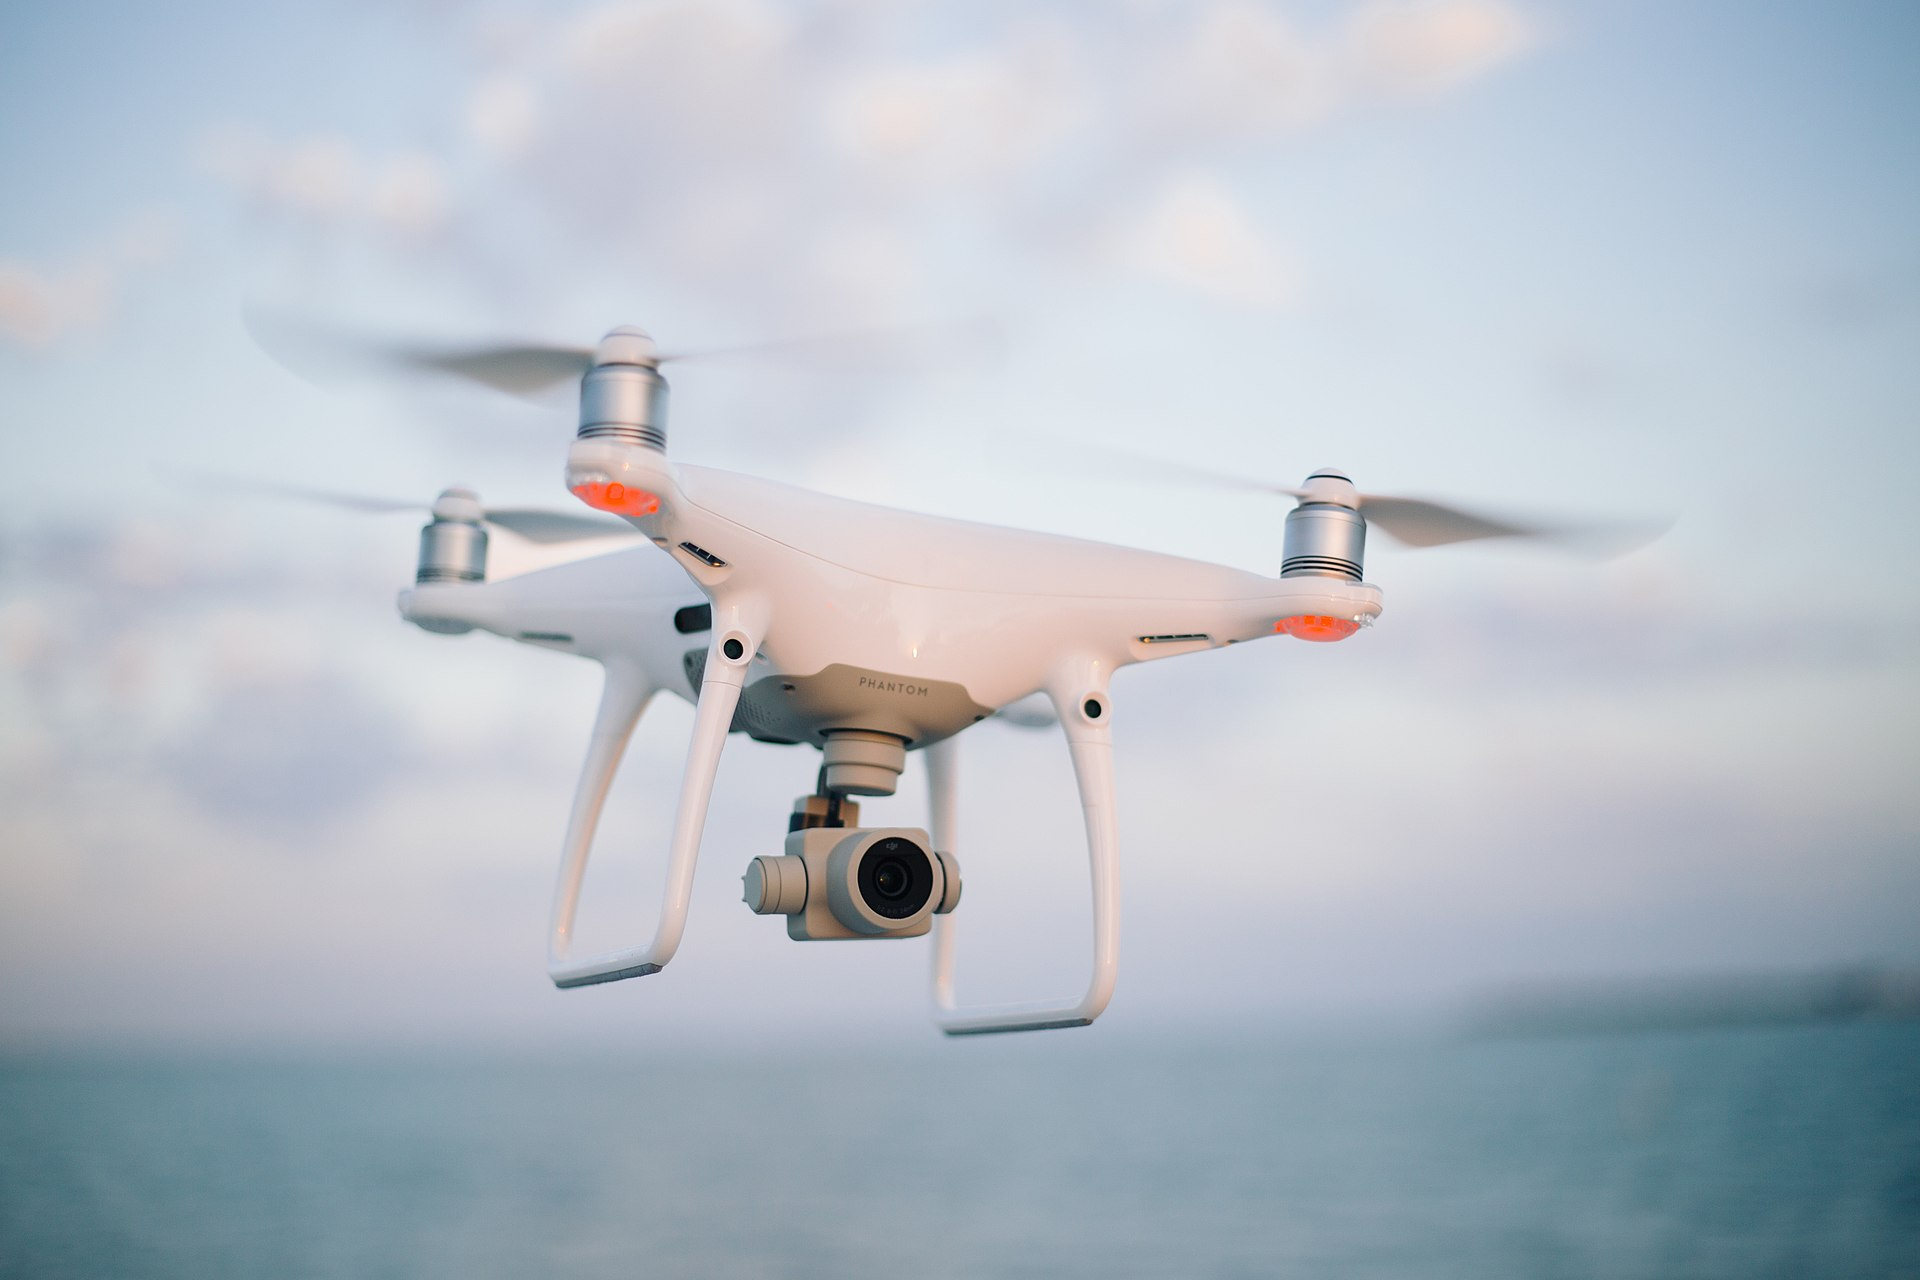
\includegraphics[width=\textwidth]{Images/Introduction/drone}
         \caption[Caption for LOF]{A DJI Phantom quadcopter (UAV)\protect\footnotemark}
         \label{fig:drone}
     \end{subfigure}
     \hfill
     \begin{subfigure}[b]{0.45\textwidth}
         \centering
         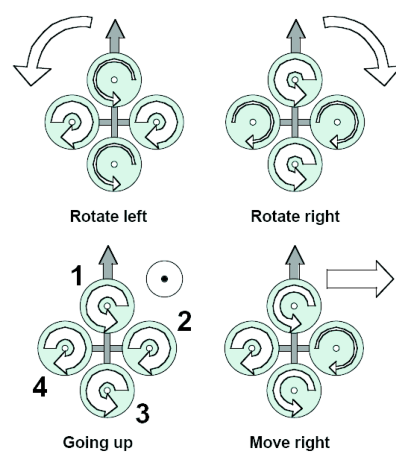
\includegraphics[width=0.6\textwidth]{Images/Introduction/propeller_direction.svg}
         \caption{Typical quadrotor configuration The width of the arrows is proportional to the angular speed of the propellers.\cite{Bouabdalla2007}}
         \label{fig:propeller_directions}
     \end{subfigure}
        \caption{A commercial quadrtotor platform, with a typical quadrotor configuration.}
        \label{fig:three graphs}
\end{figure}

The distinctive mechanical design of the quadrotor permits the actuation system to control all of the six degrees of freedom, even though it is under-actuated. This is due to the fact that the rotational and translational dynamics are tightly coupled. Thus, all the translational and rotational motions can be carried off by properly controlling the magnitude and direction of the spinning speed of the rotors.   

\footnotetext[1]{\url{https://en.wikipedia.org/wiki/Quadcopter\#/media/File:Quadcopter_camera_drone_in_flight.jpg}, accessed on 01/08/2021.}


\pagebreak

Over the last few years, quadrotors have gained a large popularity in academia and in the industry. This is due to several reasons, such as: 

\begin{enumerate}

    \item Quadrotors are very simple to design and they can be easily assembled using relatively cheap components.  
    \item As quadrotors became more and more affordable and dependable, the number of quadrotors real-world applications has grown significantly. They are being used for aerial photography, agriculture, surveillance, inspection tasks, in addition to many other uses as well. 
    \item Quadrotors are quite agile and maneuverable during flight. Especially when compared to other types of unmanned aerial vehicles (UAVs). 
    
\end{enumerate}

However, on the main challenges in the quadrotors community is the capability to design control and planning methods that will allow the quadrotors to carry out aggressive maneuvers.  The fast dynamics associated with typically small dimensions of such agile quadrotors, in addition to several aerodynamic effects that will become important during aggressive flight maneuvers, are just a few of the main problems that are faced during the system control design. Moreover, accurate tracking of the provided trajectory is a very big issue in the case of aggressive maneuvers when the rotors are commanded high speeds and accelerations, which will cause rotors to become saturated and may also cause delays.


 \section*{Parallel manipulators}

A parallel manipulator is a mechanical system that consists of two connected platforms, the fixed platform and the moving platform. The latter is linked to the fixed platform thanks to at least two serial chains that are working in parallel. When compared to serial manipulators, parallel manipulators are more accurate and rigid. In addition, the ability to install the motors next to the fixed platform is a very important feature for parallel manipulators. Moreover, parallel manipulators can be used in a wide variety of applications that demand precision and high payload combined with high speed.\cite{Parallel_Manipulators}

\begin{figure}[h]
     \centering
     \begin{subfigure}[h]{0.45\textwidth}
         \centering
         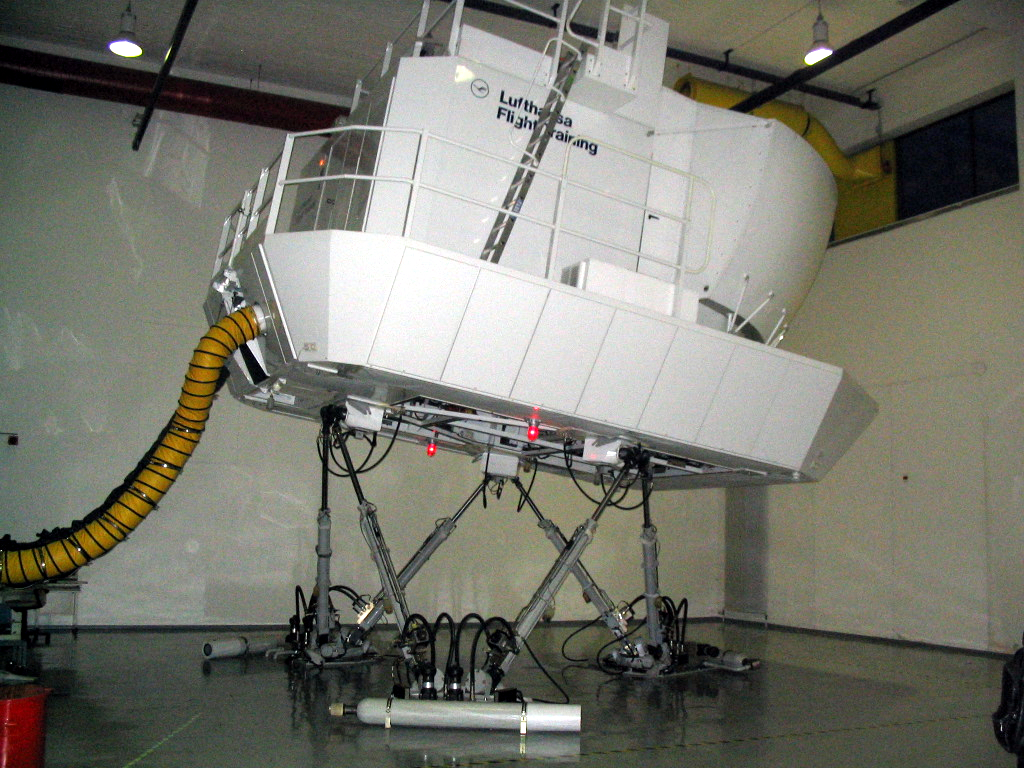
\includegraphics[width=0.7\textwidth]{Images/Introduction/GS}
    \caption[Caption for LOF]{Gough-Stewart used for a flight-simulator application.\protect\footnotemark}
         \label{GS}
     \end{subfigure}
     \hfill
     \begin{subfigure}[h]{0.45\textwidth}
         \centering
         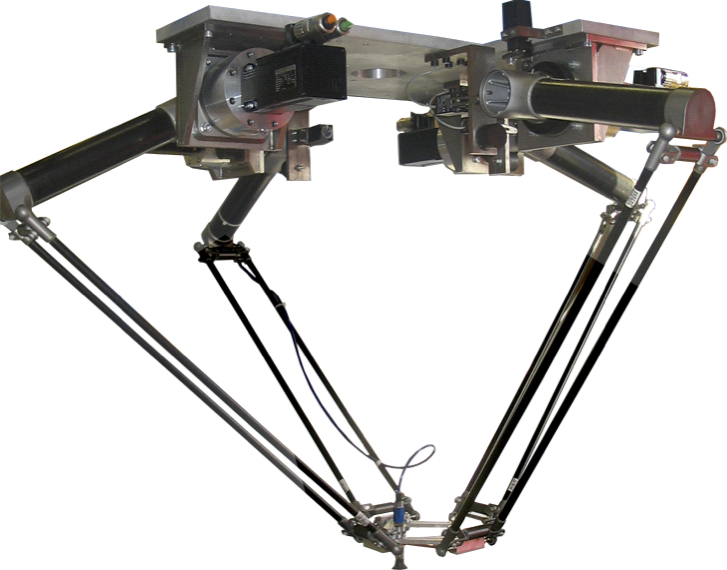
\includegraphics[width=0.7\textwidth]{Images/Introduction/PAR4}
         \caption[Caption for LOF]{The "PAR4" 4 degrees of freedom, high-speed, parallel robot prototype.\protect\footnotemark}
         \label{PAR4}
     \end{subfigure}
        \caption{Two examples of parallel robots.}
        \label{fig:three graphs}
\end{figure}




\footnotetext[1]{\url{https://en.wikipedia.org/wiki/Stewart_platform\#/media/File:Simulator-flight-compartment.jpeg}, accessed on 01/08/2021.}
\footnotetext[2]{\url{https://en.wikipedia.org/wiki/Parallel_manipulator\#/media/File:Prototype_robot_parall\%C3\%A8le_PAR4.jpg}, accessed on 01/08/2021.}


\pagebreak

However, parallel manipulators are subject to singularities, which can lead to big problems in the robot workspace in case they were not handled correctly. Thus, the study of the singular configuartions of parallel manipulators is very important. Because, even just before reaching a singularity, the performance of the parallel manipulator will decrease dramatically. Moreover, the robot may loose the ability of moving in a certain direction, gain uncontrollable motions and it the mechanism could even break. The main difference between serial and parallel manipulators is that singularity configurations may also appear inside the robot workspace (depending on the dimensions of the robot) and not just at the boundaries of the robot workspace, which can significantly decrease the area of the robot workspace.
As a result, many works have been developed by robotics researchers in order to allow parallel manipulator manipulators to safely cross these singularities by using trajectory planning and specific control methods.

\section*{The goal of this thesis}

This master thesis lies at the intersection of parallel robotics and aerial robotics. The two fields may seem very different from each other. However, quadrotors can be seen as a particular case of a parallel manipulator. 
In fact, a parallel manipulator is made up of a wrench system, applied by the robot limbs on the moving platform. And, this wrench system will define the motion of the moving platform. In the same manner, each propeller in a quadrotor can be considered as limb of a parallel robot and the moving platform to be controlled can be considered as the body of the drone. 
Specifically, the goal of this master thesis is to study a distinct class of aggressive maneuvers for quadrotors, namely multi-flip maneuvers. By doing multi-flip maneuvers, full rotations around one or more axes of the body of the quadrotor can be done. In addition, the quadrotor must also must also do the flips in a constrained environment.

\begin{figure}[h]
     \centering
     \begin{subfigure}[h]{0.45\textwidth}
         \centering
         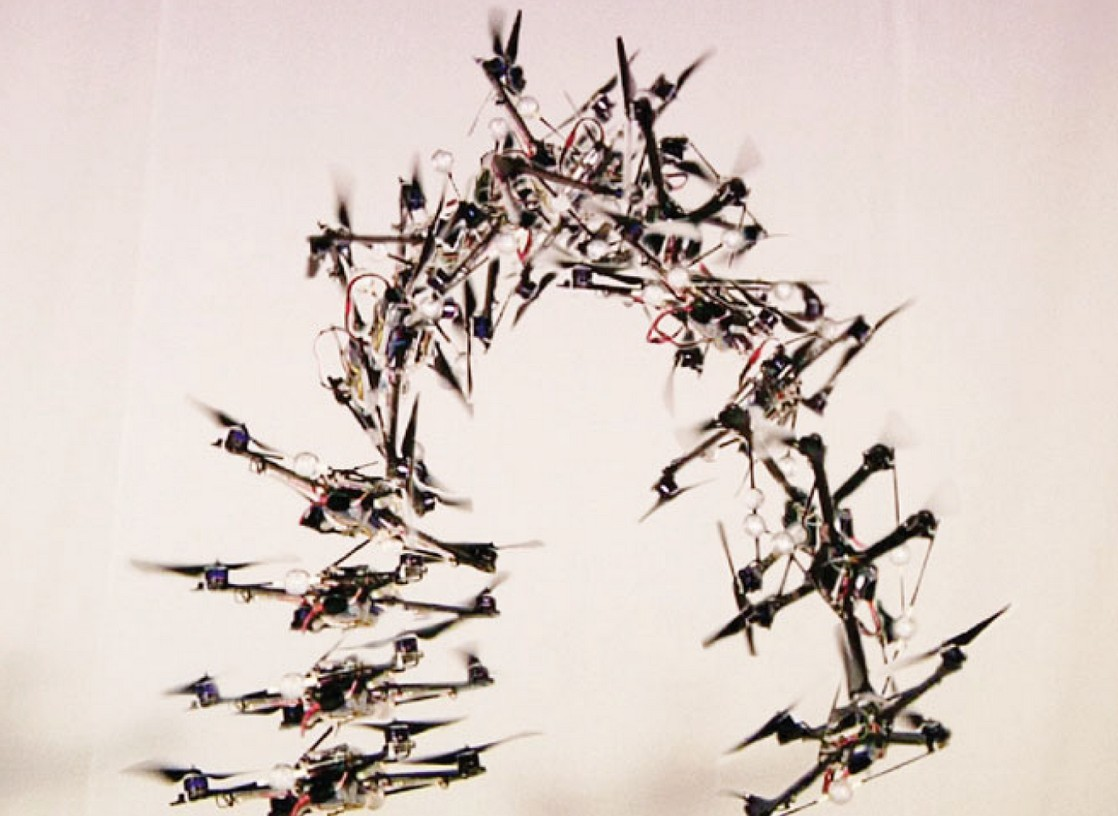
\includegraphics[width=0.9\textwidth]{Images/Introduction/flip}
    \caption{Quadrotor performing a triple flip.\cite{flip}}
         \label{triple_flip}
     \end{subfigure}
     \hfill
     \begin{subfigure}[h]{0.45\textwidth}
         \centering
         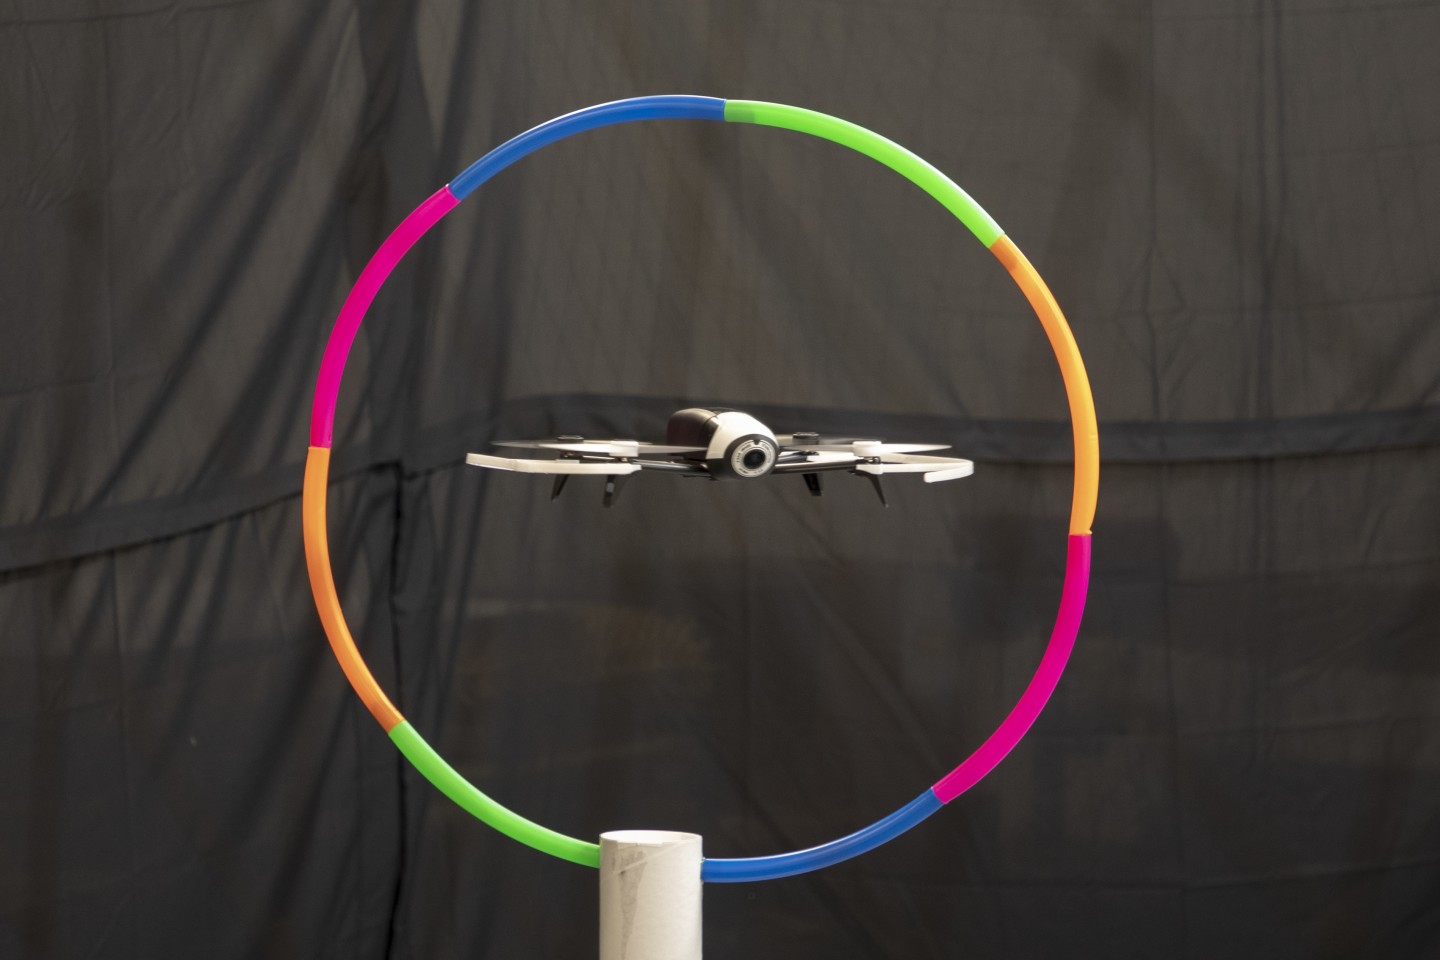
\includegraphics[width=\textwidth]{Images/Introduction/constrained_environment}
         \caption[Caption for LOF]{Quadrotor going though a loop.\protect\footnotemark[1]}
         \label{drone_hulahoop}
     \end{subfigure}
        \caption{Representation of the issues to be tackled in this master thesis.}
        \label{fig:three graphs}
\end{figure}

\footnotetext[1]{\url{https://newatlas.com/drones/muscle-signals-drone-control/\#gallery:2}, accessed on 01/08/2021.}

\pagebreak

\section*{Outline of the work}

The rest of the bibliography is structured as follows:


\begin{itemize}
\setlength{\itemindent}{-.5in}
	\item [] \textbf{Chapter 1} is devoted to introduce the system modeling of quadrotors. Specifically, a simplified dynamic model of the quadrotor will be presented by using Euler-Lagrange formalism. Then, moving on from the simple dynamic model, a more detailed dynamic model will be presented by using the Newton-Euler formalism. Finally, the state-space model of the quadrotor will also be derived.

	\item [] \textbf{Chapter 2} provides an overview of state of the art in quadrotor control in addition to introducing the different potential control methods that can be used during the master thesis in order to properly control the quadrotor. 

	\item [] \textbf{Chapter 3} provides detailed explanations of how multi-flip maneuvers can be handled. Then, the link between a quadrotor performing a flip and a parallel robot crossing a singularity will be explained. In the end, a literature review is provided in order to show how the problem is tackled by different researches.

	\item [] \textbf{Chapter 4} is devoted to trajectory optimization. By using trajectory optimization, it will be possible to create feasible trajectories for quadrotors to perform the aggressive maneuvers in constrained environments.
	
\end{itemize}

\newpage

\chapter{System Modeling}
The goal of this chapter is to present the dynamic model of the quadrotor. The mathematical notation and the physics of the quadrotor platform are expressed using the Newton-Euler formalism. Then, the state-space model that will be coded on the controller of the quadrotor will be derived.

\section{Concepts and Generalities}
The dynamic model of the quadrotor will be derived based on the following assumptions:

\begin{itemize}
	\item The quadrotor has a rigid structure.
	\item The quadrotor has a symmetrical structure.
	\item The center of gravity (CoG) and the fixed frame at the center of the body are assumed to be coincident.
	\item The propellers of the quadrotor are assumed to be rigid.
	\item The thrust and drag forces are assumed to be proportional to the square of the spinning speed of each propeller.
\end{itemize}
 
The helicopter is a complex mechanical system, it gathers many physical effects from the domain of mechanics and aerodynamics \cite{houston_2001}. Thus, all the significant effects including the gyroscopic effects must be considered in the modeling of the quadrotor. A small list of the most important effects that a helicopter is subject to \cite{Mullhaupt1999} are briefly described in table \ref{physical_effects}:

\begin{table}[h]
\caption{The main physical effects that the helicopter is subject to. }\label{physical_effects}
\centering
\setlength{\tabcolsep}{10pt} % Default value: 6pt
\renewcommand{\arraystretch}{1} % Default value: 1
\begin{tabular}{c c c}
\hline
\hline
Effect & Source & formulation \\
\hline
Aerodynamic effects & \shortstack{Rotation of propeller \\ Flapping of blades} & $C \Omega^2$\\
\hline
Inertial counter torques & \shortstack{Change in propeller \\ spinning speed} & $ J \dot{\Omega}$\\
Gravitational effect & Position of the center of mass & {} \\
\hline
Gyroscopic effects & \shortstack{Orientation change  \\ of the rigid body} & $ I \theta \psi$\\
 {} & \shortstack{Orientation change  \\ of the propeller plane} & $ J \Omega_r \theta,\phi$ \\
 \hline
Friction & All helicopter motions & $C \dot{\phi},\dot{\theta},\dot{\psi}$\\
\hline
\hline
\end{tabular}
\end{table}

\newpage 

 \section{Modelling with Euler-Lagrange Formalism} 
 The dynamics of the rotation of a simple quadrotor are modeled using the Euler-Lagrange Formalism in this section. A fixed frame $E$ for the world frame and body fixed frame $B$ for the quadrotor are considered as represented in figure \ref{coordinate_system_simple}. The orientation of the quadrotor frame in space is provided by a rotation $R$ from $B$ to $E$, where $R\in SO3$ is a $3 \times 3 $ rotation matrix.
 
 
 \begin{figure}[h]
 \centering
 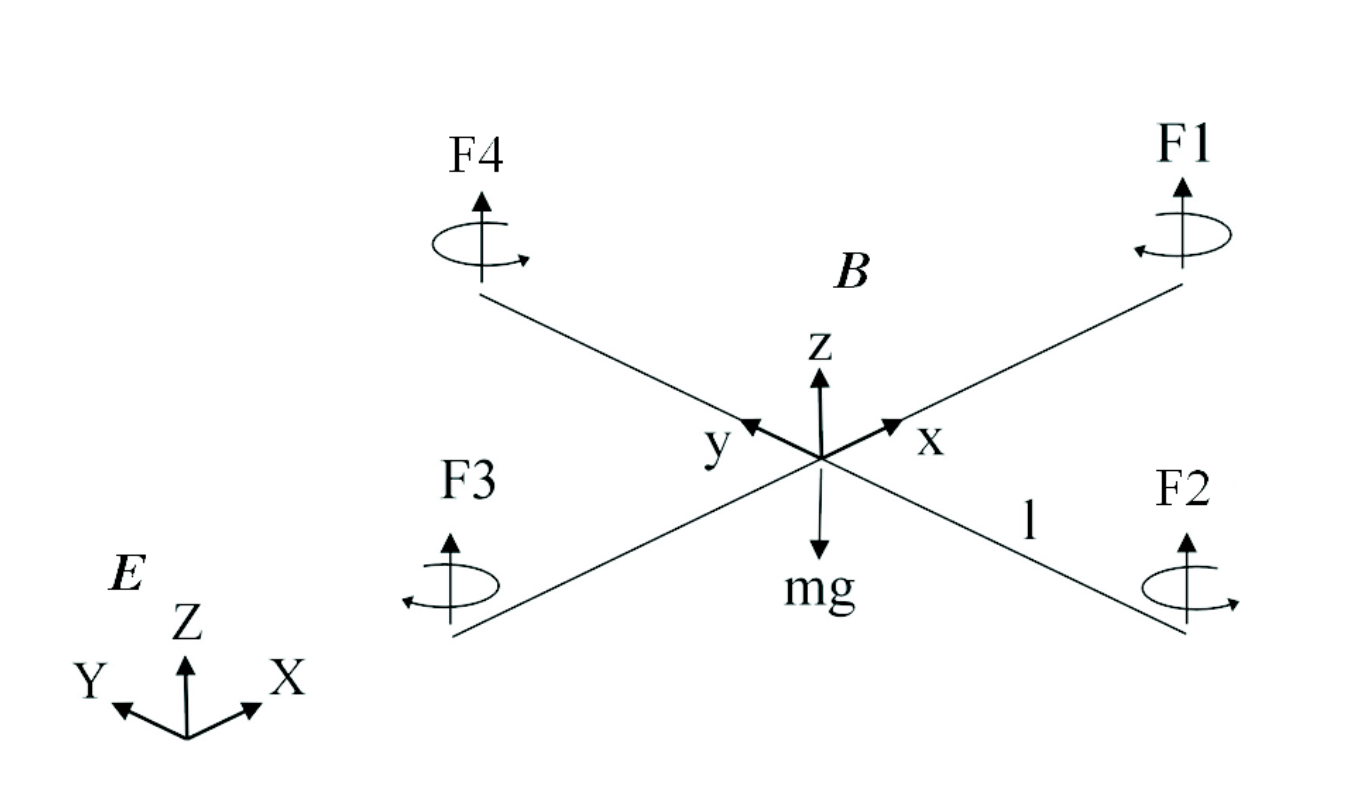
\includegraphics[width=0.5\textwidth]{Images/Modeling/Test_Bench}
 \caption{Simplified coordinate system of a quadrotor. \cite{Bouabdalla2007}}
 \label{coordinate_system_simple}
 \end{figure}

\subsection{Kinematics} 
 
 For any point of the body frame of the quadrotor expressed in the fixed world frame, the following can be written 
 ( c: $\cos$, s: $\sin$):   
 
 \begin{equation}\label{kinematics}
 \begin{cases}
 r_X= (c\psi c \theta ) x + ( c \psi s \theta s \phi  - s \psi c \phi) y + (c \psi s \theta c \phi + s \psi s \phi) z \\
 \\
 r_Y= (s\psi c \theta ) x + ( s \psi s \theta s \phi  + c \psi c \phi) y + (s \psi s \theta c \phi - c \psi s \phi) z \\
 \\
 r_Z= (-s \theta ) x + ( c \theta s \phi ) y + (c \theta c \phi) z \\ 
 \end{cases}
 \end{equation}

Thus, the velocities can be derived by differentiation \ref{kinematics}, and the squared magnitude of the squared velocity can be expressed as follows for any point:

\begin{equation}\label{velocity_magnitude}
	v^2 = v_X^2 + v_Y^2 + v_Z^2\\
\end{equation} 

\subsection{Energy}

Assuming that the matrix of inertia is diagonal, then from equation \ref{velocity_magnitude}, the expression of the kinetics energy can be calculated:

\begin{equation}\label{kinetic_energy}
T = \frac{1}{2} I_{xx}(\dot{\phi}-\dot{\psi} s \theta)^2 + \frac{1}{2} I_{yy}(\dot{\theta} c \phi + \dot{\psi} s \phi c \theta)^2 + \frac{1}{2} I_{zz}(\dot{\theta} s \phi - \dot{\psi} c \phi)^2
\end{equation}

Using the formula of the potential energy, equation \ref{kinetic_energy} can be expressed in the fixed world frame as: 

\begin{equation}\label{potential_energy}
V = \int xdm(x)(-g s \theta) + \int ydm(y)(g s \phi c \theta) + \int z dm (z) (g c \phi c \theta) 
\end{equation}

\newpage

\subsection{Equation of Motion}

By using the Euler-Lagrange formalism:


\begin{equation}
L = T - V \text{\hspace{0.5cm} ,\hspace{0.5cm}} \Gamma_i = \frac{d}{dt}\bigg(\frac{\partial L}{\partial \dot{q}_i}\bigg) - \frac{\partial L}{\partial q_i}
\end{equation}
 
 Where $L$ $\Gamma_i$ and $\dot{q}_i$ are the Lagrangian, the generalized forces and the generalized coordinates respectively. Thus, the equations of motion can be expressed as follows: 
 
 \begin{equation}
 \begin{cases}
 I_{xx}\ddot{\phi} = \dot{\theta} \dot{\psi}(I_{yy}-I_{zz})\\
 \\
 I_{yy}\ddot{\theta} = \dot{\phi} \dot{\psi}(I_{zz}-I_{xx})\\
 \\
 I_{zz}\ddot{\psi} = \dot{\phi} \dot{\theta} (I_{xx} - I_{yy})
 \end{cases}
 \end{equation}
 
Moreover, the torques that are nonconservative and acting on the quadrotor, are due to two different causes. First, it is due to thrust of each rotor pairs in figure \ref{coordinate_system_simple}:

\begin{equation}
\begin{cases}
\tau_x = bl(\Omega_4^2 - \Omega_2^2)\\
\\
\tau_y = bl(\Omega_3^2 - \Omega_1^2)\\
\\
\tau_z = bl(\Omega_1^2 - \Omega_2^2 + \Omega_3^2 - \Omega_4^2)\\
\end{cases}
\end{equation}

Second, it is also due to the gyroscopic effect which is the result of the rotation of the propellers:

\begin{equation}
\begin{cases}
\tau_x' = J_r \omega_y (\Omega_1 + \Omega_3 - \Omega_2 - \Omega_4)\\
\\
\tau_y' = J_r \omega_x (\Omega_2 + \Omega_4 - \Omega_1 - \Omega_3)\\
\end{cases}
\end{equation}

\subsection{The Derived Dynamic Model}

The dynamic model of the quadrotor which describes the rotations of roll, pitch and yaw consists of three terms:
\begin{enumerate}
	\item The actuator torques.
	\item The gyroscopic effects that are due to the rotation of the rigid body.
	\item The gyroscopic effects that are due to rotation of the propeller that is coupled with the rotation of the body.
\end{enumerate}

 Thus, the dynamic model of the quadrotor is:
 
 \begin{equation}\label{dynamic_model}
 	\begin{cases}
 		I_{xx}\ddot{\phi}= \dot{\theta}\dot{\psi}(I_{yy}-I_{zz})-J \dot{\theta} \Omega_r + \tau_x \\
 		\\
 		I_{yy}\ddot{\theta}= \dot{\theta}\dot{\psi}(I_{zz}-I_{xx})+J \dot{\phi} \Omega_r + \tau_y \\
 		\\
 		I_{zz}\ddot{\psi}= \dot{\phi}\dot{\theta}(I_{xx}-I_{yy}) + \tau_z \\	
 	\end{cases}
 \end{equation}

 
 
 \newpage
 
 \subsection{Rotor Dynamics}
 
 DC motors are used to drive the rotors of a quadrotor. So, the established equations of a DC motor are the following:

\begin{equation}\label{DC_motor_dynamics}
\begin{cases}
L \frac{di}{dt}=u - R_{mot}i - k_e \omega_m\\
\\
J_m \frac{d \omega_m}{dt} = \tau_m - \tau_d \\
\end{cases}
\end{equation} 

Since small motors are used in which they also have little inductance, then the second order equation of the DC motor dynamics is given by:

\begin{equation}\label{DC_motor_2nd_order_dynamics}
	J_m \frac{d\omega_m}{dt} = -\frac{k_m^2}{R_{mot}}\omega_m - \tau_d + \frac{k_m}{R_{mot}}u
\end{equation}
 
When the gearbox and the propeller models are introduced, then equation \ref{DC_motor_2nd_order_dynamics} becomes:

\begin{equation}\label{DC_motor_2nd_order_dynamics}
\begin{cases}
	\dot{\omega}_m = - \frac{1}{\tau}\omega_m - \frac{d}{\eta r^3 J_t}\omega_m^2 + \frac{1}{k_m \tau}u\\
	\\
	\frac{1}{\tau} = \frac{k_m^2}{RJ_t}\\
	\end{cases}
\end{equation}
 
Moreover, linearization of equation \ref{DC_motor_2nd_order_dynamics} can be done around an operation point $\dot{\omega}_0$ to the form $\dot{\omega}_m = -A \omega_m + B u + C$ with: 

\begin{equation}
A = \bigg( \frac{1}{\tau}+\frac{2d\omega_0}{\eta r^3 J_t} \bigg) \text{ \hfill , \hfill} B = \bigg( \frac{1}{k_m \tau} \bigg) \text{\hfill , \hfill} C = \bigg( \frac{d \omega_0^2}{\eta r^3 J_t} \bigg)
\end{equation}
 
 
 \section{Modeling with Newton-Euler Formalism}
 
The model above was derived in succession as shown in papers  \cite{Bouabdallah2004,Bouabdallah2005a,Bouabdallah2005b} . The dynamic equations below include rolling moments $R_m$, hub forces $H$ and various aerodynamic effects.
Thus, this is a more realistic dynamic model, especially when the quadrotor flies in a forward manner. 
With the previous versions of the dynamic model, it was required to to moderately tune the control parameters in order to have experiments that are successful.

The dynamic model expressed in the Newton-Euler formalism of a rigid body that is subject to external forces acting on the center of mass  \cite{Murray1994} is expressed as follows:

\begin{equation}\label{NE_Formalism}
\begin{bmatrix}
m I_{3 \times 3} && 0 \\
0 && I \\
\end{bmatrix}
\begin{bmatrix}
\dot{V}\\
\dot{\omega}\\
\end{bmatrix}
+ \begin{bmatrix}
\omega \times mV \\
\omega \times I \omega \\
\end{bmatrix}
=
\begin{bmatrix}
F \\
\tau \\
\end{bmatrix}
\end{equation}
 
Considering a fixed world frame $E$ and a fixed body frame $B$ on the quadrotor as shown in figure \ref{coordinate_system_detailed_quadrotor}. Then, by the use of the Euler angles, the orientation of the rigid body of the quadrotor in space is expressed by a rotation $R$ from $B$ to $E$, where $R \in SO3$ is a rotation matrix. 
 
 \begin{figure}[h]
\centering
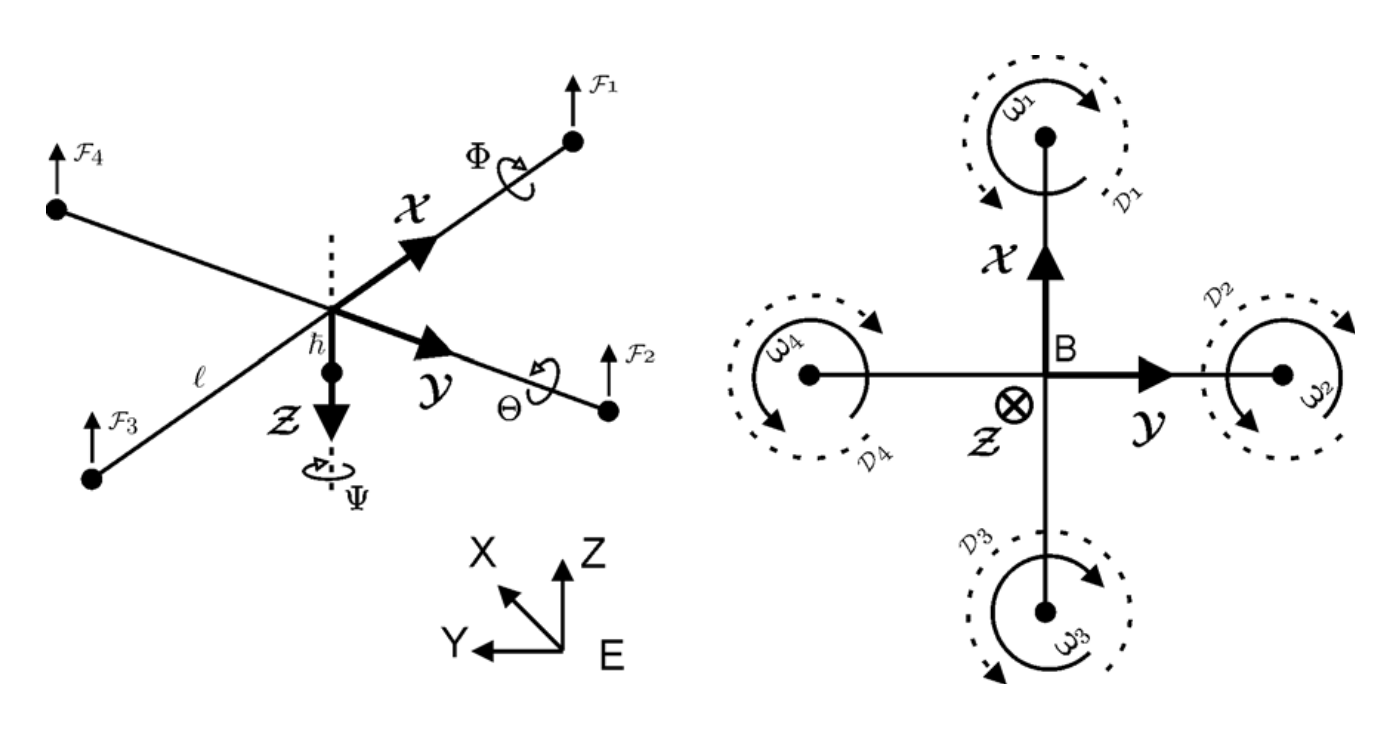
\includegraphics[width=0.5\textwidth]{Images/Modeling/Detailed_quadrotor}
\caption{Detailed coordinate system showing the forces with the roll, pitch and yaw angles (left) and the moments (right) applied on a quadrotor. \cite{Bouabdalla2007}}
\label{coordinate_system_detailed_quadrotor}
\end{figure}
 
\newpage

\subsection{Aerodynamic Forces and Moments}

The aerodynamic forces and moments are computed using a mix of blade element and momentum theory \cite{Leishmana}. This is based off of the work of Gary Fay during the project of the Mesicopter \cite{Leishmanb}. For a simpler readings of the equations provided below, some symbols are recalled:

\begin{table}[h]
\centering
\setlength{\tabcolsep}{10pt} % Default value: 6pt
\renewcommand{\arraystretch}{1} % Default
\begin{tabular}{c c}
$\sigma$: solidity ration & $\lambda$: inflow ratio \\
$a$: lift slope & $v$: induced velocity \\
$\mu$: rotor advance ration & $\rho$: air density

\end{tabular}
\captionsetup[table]{list=no}
\end{table}
 
\subsubsection*{Thrust Force}

The thrust force is due to all the vertical forces that the blade elements are subject to.

\begin{equation}\label{thrust_force}
\begin{cases}
T = C_T \rho A(\Omega R_{rad})^2\\
\\
\frac{C_T}{\sigma a} = (\frac{1}{6} + \frac{1}{4} \mu^2)\theta_0 - (1+\mu^2)\frac{\theta_{tw}}{8} - \frac{1}{5} \lambda \\
\end{cases}
\end{equation}

\subsubsection*{Hub Force}

The hub force is due to all the horizontal forces that the blade elements are subject to.

\begin{equation}
\begin{cases}
H = C_H \rho A(\Omega R_{rad})^2\\
\\
\frac{C_H}{\sigma a} = (\frac{1}{4a} \mu \overline{C_d} + \frac{1}{4} \lambda \mu (\theta_0 - \frac{\theta_{tw}}{2})\\
\end{cases}
\end{equation}

\subsubsection*{Drag Moment}

The drag moment about the rotor shaft is due to the aerodynamic forces that the blade elements are subject to. The horizontal forces that are acting on the rotor are multiplied by the moment arm and  integrated over the rotor. The drag moment gives the required power to spin the rotor.

\begin{equation}
\begin{cases}
	Q = C_Q \rho A (\Omega R_{rad})^2 R_{rad}\\
	\\
	\frac{C_Q}{\sigma a} = \frac{1}{8a}(1+\mu^2) \overline{C_d} + \lambda (\frac{1}{6} \theta_0 - \frac{1}{8} \theta_{tw} - \frac{1}{4} \lambda)
\end{cases}
\end{equation}

\newpage

\subsubsection*{Rolling moment}


The rolling moment of a propeller occurs when the blade that is advancing is producing more lift than the blade that is retreating in forwarding flight. It is the integration of the lift of every single section that is acting at a given radius over the entire rotor.
The reader should notice that the rolling moment is not the same as the propeller radius, or the overall rolling moment which is due to other effects or the rotation matrix $R$. So, there should not be any confusion.

\begin{equation}
\begin{cases}
R_m = C_{R_m}\rho A (\Omega R_{rad})^2 R_{rad} \\
\\
\frac{C_{R_m}}{\sigma a} = -\mu (\frac{1}{6} \theta_0 - \frac{1}{8} \theta_{tw} - \frac{1}{8} \lambda)\\
\end{cases}
\end{equation}

\subsubsection*{Ground Effect}


When operating near the ground ( at a height equivalent to half the diameter of the rotor), helicopters experience thrust augmentation which is caused by greater efficiency of the rotor.This is linked to a decrease in the velocity of induced airflow. Moreover, this is called Ground Effect. Different approaches to deal with this effect can be found in literature, for example, adaptive techniques can  be used \cite{Guenard2006}.
However, the objective is to find a model that is simple and mainly captures the change in the velocity of the induced inflow.
Cheeseman \cite{Cheeseman1957} states (reached from the images method \cite{Griffiths2002}) that if the power is constant ($T_{OGE}v_{i,OGE} = T_{IGE}v_{i,IGE}$), the generated vecolity at the center of the rotor by its imageis $\delta v_i = Av_i/16 \pi z^2$.
Cheesman acquired the relation (\ref{Cheeseman}) by using the assumption that both $v_i$ and $\delta v_i$ are constant over disk, which results in $v_{i,IGE}=v_i-\delta v_i$.

\begin{equation}\label{Cheeseman}
\frac{T_{IGE}}{T_{OGE}}=\frac{1}{1-\frac{R^2_{rad}}{16 z^2}}
\end{equation}

An alternative way to move forward is to consider that the inflow ration of the inflow ratio is $\lambda_{IGE} = (v_{i,OGE}-\delta v_i - \dot{z})/\Omega R_{rad}$, where the change of the velocity of the induced inflow is $\delta v_i = v_i/(4z/R_{rad})^2$.Then, the thrust coefficient (\ref{thrust_force}) IGE can be rewritten  as:

\begin{equation}
\begin{cases}
T_{IGE}=C_T^{IGE} \rho A(\Omega R_{rad})^2 \\
\\
\frac{C_T^{IGE}}{\sigma a} = \frac{C_T^{OGE}}{\sigma a} + \frac{\delta v_i}{4 \Omega R_{rad}}\\
\end{cases}
\end{equation} 


\newpage

\subsection{General Moments and Forces}\label{forces_and_moments}

The motion of the quadrotor is the result of several forces and moments that are originating from different physical effects \cite{Bouabdalla2007}. In this model, the following effects are considered (with $c$: $\cos$, $s$:$\sin$).

\subsubsection*{Rolling Moments}

\setlength{\tabcolsep}{20pt}
 \begin{tabular}{lp{0.8\textwidth}}
  body gyro effect & $\dot{\theta}\dot{\psi}(I_{yy}-I_{zz})$\\
  \\
  propeller gyro effect & $J_r \dot{\theta}\Omega_r$\\
  \\
  pitch actuators action & $l(-T_2+T_4)$\\
  \\
  hub moment due to forward flight & $h(\sum_{i=1}^4 H_{yi})$\\
  \\
  rolling moment due to forward flight & $(-1)^{i+1}\sum_{i=1}^4 R_{mxi}$\\
  \\
\end{tabular}

\subsubsection*{Pitching Moments}

\setlength{\tabcolsep}{20pt}
 \begin{tabular}{lp{0.8\textwidth}}
 body gyro effect & $\dot{\phi}\dot{\psi}(I_{zz}-I_{xx})$\\
 \\
 propeller gyro effect & $J_r \dot{\phi}\Omega_r$ \\
 \\
 pitch actuators action & $l(T_1-T_3)$\\
 \\
 hub moment due to forward flight & $h(\sum_{i=1}^4 H_{xi})$\\
 \\
 rolling moment due to side-ward flight &  $(-1)^{i+1}\sum_{i=1}^4 R_{myi}$\\
\end{tabular}

\subsubsection*{Yawing Moments}

\setlength{\tabcolsep}{20pt}
 \begin{tabular}{lp{0.8\textwidth}}
body gyro effect & $\dot{\theta}\dot{\phi}(I_{xx}-I_{yy})$\\
\\
inertial counter-torque & $J_r \dot{\Omega}_r$\\
\\
counter-torque unbalance & $(-1)^i\sum_{i=1}^4 Q_i$\\
\\
hub force unbalance in forward flight & $l(H_{x2}-H_{x4})$ \\
\\
hub force unbalance in sideward flight & $l(-H_{y1}+H_{y3})$\\

\end{tabular}


\subsubsection*{Forces Along z Axis}

%
\setlength{\tabcolsep}{58pt}
 \begin{tabular}{lp{1\textwidth}}
actuators action & $c \psi c \phi (\sum_{i=1}^4T_i$\\
\\
weight & $mg$ \\

\end{tabular}

\subsubsection*{Forces Along x Axis}
\setlength{\tabcolsep}{58pt}
 \begin{tabular}{lp{1\textwidth}}
actuators action & $ (s \psi s \phi + c \psi s \theta c \phi)(\sum_{i=1}^4 T_i) $\\
\\
hub force in x axis & $-\sum_{i=1}^4 H_{xi}$ \\
\\
friction & $\frac{1}{2}C_x A_c \rho \dot{x}|\dot{x}|$

\end{tabular}


\subsubsection*{Forces Along y Axis}
\setlength{\tabcolsep}{58pt}
 \begin{tabular}{lp{1\textwidth}}
actuators action & $ (-c \psi s \phi + s \psi s \theta c \phi)(\sum_{i=1}^4 T_i) $\\
\\
hub force in y axis & $-\sum_{i=1}^4 H_{yi}$ \\
\\
friction & $\frac{1}{2}C_y A_c \rho \dot{y}|\dot{y}|$

\end{tabular}

\subsection{Equations of Motion}\label{detail_equation_of_motin}

The equations of motion are derived from (\ref{NE_Formalism}) in addition to all the forces and the moments that were listed in subsection \ref{forces_and_moments}.

\begin{equation}\label{detailed_dynamic_model}
\begin{cases}
I_{xx}\ddot{\phi} = \dot{\theta} \dot{\psi}(I_{yy}-I_{zz}) + J_r \dot{\theta}\Omega_r + l(-T_2+T_4)-h(\sum_{i=1}^4H_{yi})+(-1)^{i+1} \sum_{i=1}^4 R_{mxi}\\
\\
I_{yy}\ddot{\theta} = \dot{\phi} \dot{\psi}(I_{zz}-I_{xx}) - J_r \dot{\phi}\Omega_r + l(T_1-T_3) + h(\sum_{i=1}^4H_{xi})+(-1)^{i+1} \sum_{i=1}^4 R_{mxi}\\
\\
I_{zz}\ddot{\psi} = \dot{\phi} \dot{\psi}(I_{xx}-I_{yy}) + J_r \dot{\Omega}_r +(-1)^i \sum_{i=1}^4 Q_i + l(H_{x2}-H_{x4})+l(-H_{y1}+H_{y3})\\
\\
m\ddot{z} = mg -(c \psi c \phi)\sum_{i=1}^4T_i\\
\\
m\ddot{x} = (s \psi s \phi + c \psi s \theta c \phi) \sum_{i=1}^4 T_i - \sum_{i=1}^4 H_{xi}-\frac{1}{2}C_xA_c \rho \dot{x}|\dot{x}|\\
\\
m \ddot{y} = ( - c \psi s \phi + s \psi s \theta c \phi) \sum_{i=1}^4 T_i - \sum_{i=1}^4H_{yi} - \frac{1}{2}C_y A_c \rho \dot{y}|\dot{y}|\\
\end{cases}
\end{equation}

\newpage


 \section{State-Space Model}
The model \ref{detailed_dynamic_model} that was developed in subsecton \ref{detail_equation_of_motin} expresses the differential equations of the system. However, for the purpose of control design, it is desirable to reduce the complexity and simplify the model to satisfy the real-time limitations of the embedded control loop. Thus, the thrust and the drag coefficients are assumed to be constant and the hub forces and rolling moments are neglected. As a result, the system can be expressed in state-space form \\ $\dot{\textbf{\textsc{x}}}=f(\textbf{\textsc{x}},\textbf{\textsc{u}})$ with $\textbf{\textsc{x}}$ the state vector and $\textbf{\textsc{u}}$ the control input vector.

The state vector has the following form:

\begin{equation}\label{state_vector}
\textbf{\textsc{x}} = \left[\begin{array}{c c c c c c c c c c c c c}
\phi & \dot{\phi} & \theta & \dot{\theta} & \psi & \dot{\psi} & z & \dot{z} & x & \dot{x} & y & \dot{y} 
\end{array}\right]^{\intercal}
\end{equation}
  
 With,
 
\begin{multicols}{2}
 
\begin{equation*}
\begin{aligned}
x_1 = \phi\\
x_2 = \dot{x}_1=\dot{\phi}\\
x_3 = \theta\\
x_4 = \dot{x}_3 = \dot{\theta} \\
x_5 = \psi \\
x_6 = \dot{x}_5 = \dot{\psi}\\
\end{aligned}
\end{equation*}

\columnbreak

\begin{equation}
\begin{aligned}
x_7 = z\\
x_8 = \dot{x}_7=\dot{z}\\
x_9 = x\\
x_{10} = \dot{x}_9 = \dot{x} \\
x_{11} = y \\
x_{12} = \dot{x}_{11} = \dot{y}\\
\end{aligned}
\end{equation}

\end{multicols}
 
Moreover, the control input vector has the following form: 

\begin{equation}\label{control_input_vector}
\textbf{\textsc{u}} = \left[\begin{array}{c c c c}
u_1 & u_2 & u_3 & u_4 
\end{array}\right]^{\intercal}
\end{equation}

Where the control inputs are mapped by: 

\begin{equation}\label{Control_input_mapping}
\begin{cases}
u_1 = b(\Omega_1^2 + \Omega_2^2 + \Omega_3^2 + \Omega_4^2)\\
\\
u_2 = b(-\Omega_2^2 + \Omega_4^2)\\
\\
u_3 = b(\Omega_1^2 - \Omega^3)\\
\\
u_4 = d(-\Omega_1^2 + \Omega_2^2 - \Omega_3^2 + \Omega_4^2) \\
\end{cases}
\end{equation}

The transformation matrix between the rate change of the attitude angles ($\dot{\phi},\dot{\theta},\dot{\psi}$) and the angular velocities of the body($p,q,r$) can be regarded as the identity matrix if the disturbances due to hover flight are small. As a result, the following can be written:

\begin{equation}
(\dot{\phi},\dot{\theta},\dot{\psi})  \approx (p,q,r)
\end{equation}

Simulation tests have demonstrated that this assumption is reasonable \cite{Bouabdalla2007}. 

\newpage

From equations (\ref{detailed_dynamic_model}),(\ref{state_vector}),(\ref{control_input_vector}), the following expression is obtained after simplification:

\begin{equation}\label{state_space_model}
f(\textbf{\textsc{x}},\textbf{\textsc{u}}) = \begin{pmatrix}
\dot{\phi}\\
\dot{\theta} \dot{\psi} a_1 + \dot{\theta} a_2 \Omega_r + b_1 u_2 \\
\dot{\theta}\\
\dot{\phi} \dot{\psi} a_3 - \dot{\phi} a_4 \Omega_r + b_2 u_3 \\
\dot{\psi}\\
\dot{\theta} \dot{\psi} a_5 + b_3 u_4 \\
\dot{z}\\
g - (\cos \phi \cos \theta) \frac{1}{m} u_1 \\
\dot{x} \\
u_x \frac{1}{m} u_1\\
\dot{y}\\
u_y \frac{1}{m}u_1\\
\end{pmatrix}
\end{equation}

With, 

\begin{multicols}{2}
 
\begin{equation*}
\begin{aligned}
a_1 &= (I_{yy} - I_{zz})/I_{xx}\\
a_2 &= J_r/I_{xx}\\
a_3 &= (I_{zz} - I_{xx})/I_{yy}\\
a_4 &= J_r/I_{yy}\\
a_5 &= (I_{xx} - I_{yy})/I_{zz}\\
\end{aligned}
\end{equation*}

\columnbreak

\begin{equation}
\begin{aligned}
b_1 &= l/I_{xx}\\
b_2 &=l/I_{yy}\\
b_3 &= l/I_{zz}\\
\end{aligned}
\end{equation}

\end{multicols}

\begin{equation}
	\begin{aligned}
	u_x = (\cos \phi \sin \theta \cos \psi + \sin \phi \sin \psi)\\
	u_y = (\cos \phi \sin \theta \sin \psi - \sin \phi \cos \psi)\\
	\end{aligned}
\end{equation}

It is important to note that that the angles and the derivatives of the angles do not depend on the components of the translation in the system represented by equation (\ref{state_space_model}). Contrarily, the translation components depend of the angles. So, the system represented by equation(\ref{state_space_model}) can be depicted as two subsystems, the angle subsystem and the translation subsystem as shown in figure 

\begin{figure}[h]
\centering 
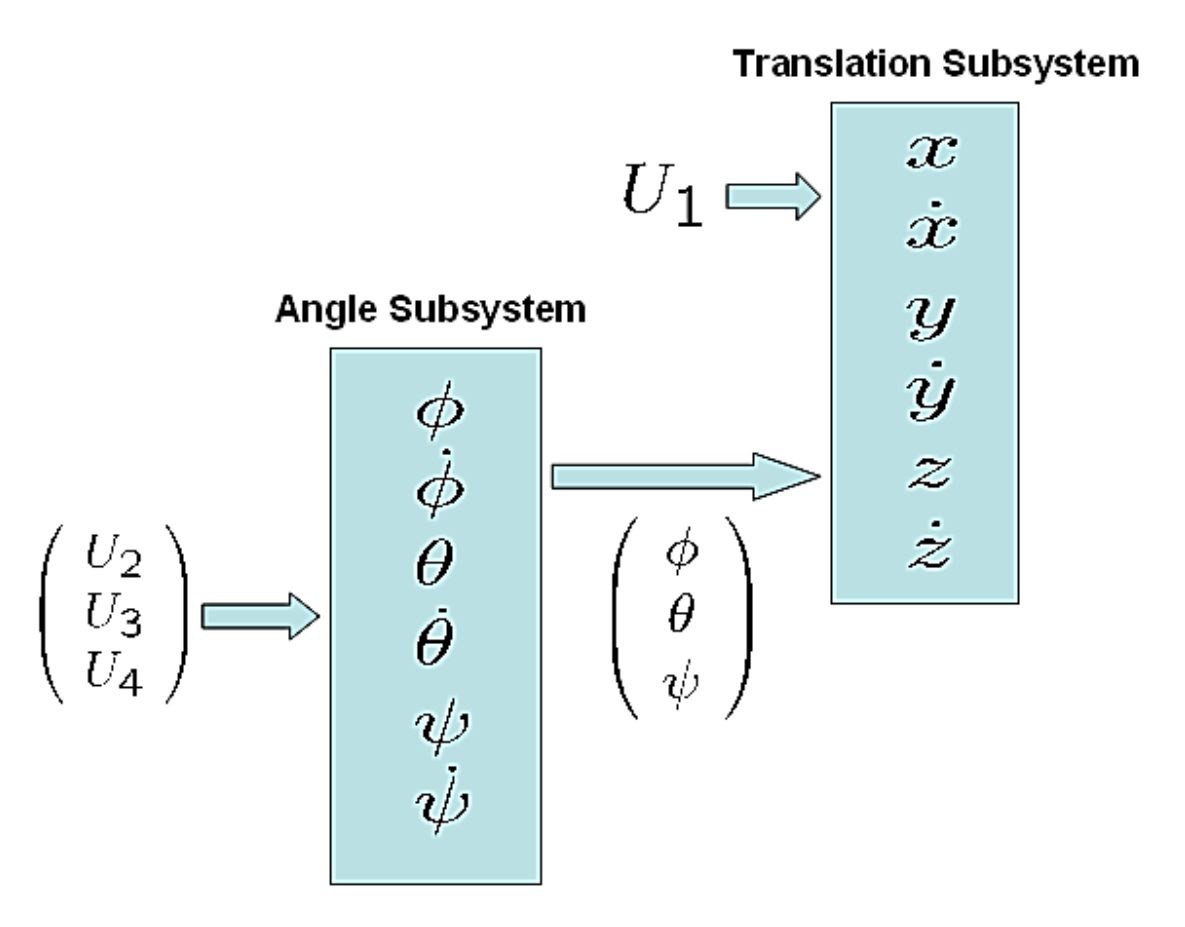
\includegraphics[width=0.5\textwidth]{Images/Modeling/subsystems}
\caption{Link between the rotation and the translation subsystems.\cite{Bouabdalla2007}}
\end{figure}

 \chapter{Control of quadrotors}
In the following sections of this chapter, differential flatness,  the general control architecture of a quadrotor and different potential control approaches (linear and nonlinear) that can be used to control a quadrotor are explained. 
 \section{Differential Flatness}\label{Differential_flatness}  
 
 In the quadrotor community, a well-established finding is that the dynamic model of a quadrotor is differentially flat. Moreover, the control design problem in non-linear systems will be considerably simplified. Precisely, a system with state $\textbf{\textsc{x}} \in \mathbb{R}^n$ and input $\textbf{\textsc{u}} \in \mathbb{R}^m$ is considered to be \textit{differentially flat} if there exists a set of \textit{flat outputs} $\textbf{\textsc{y}} \in \mathbb{R}^m$ which have the following form:
 
 \begin{equation}
 \textbf{\textsc{y}} = \textbf{\textsc{y}}(\textbf{\textsc{x}}, \textbf{\textsc{u}}, \dot{\textbf{\textsc{u}}},...,\textbf{\textsc{u}}^{(p)})
 \end{equation}

 With, 
 
 \begin{equation}
 	\begin{cases}
 		\textbf{\textsc{x}} = \textbf{\textsc{x}}(\textbf{\textsc{y}}, \dot{\textbf{\textsc{y}}},...,\textbf{\textsc{y}}^{(q)}) \\
 	\\
 		\textbf{\textsc{u}} = \textbf{\textsc{u}}(\textbf{\textsc{y}}, \dot{\textbf{\textsc{y}}},...,\textbf{\textsc{y}}^{(r)}) \\
 	\end{cases}
 \end{equation}

 Thus, the new set of variables is required to be a function of the state, the input and the derivatives of the input. Moreover, this set should also have the same dimensions as the control input. In this manner, it is possible to rewrite both the state and the input in function of the flat outputs and the derivatives of the flat outputs.This is a very useful property in underactuated systems where $m<n$, such as quadrotors, because, it will allow to generate trajectories in the lower dimensional space $m$, then this trajectory will be mapped into the full dimensional \\ space $n$. Another well known example of systems is a car, in which the underactuation is the result of the nonholonomic constraints that are imposed by the wheels. So, for a car, a generated trajectory for $(x,y)$ position of the rear-wheels is enough to specify all the viable trajectories of the system.Formal proofs that the quadrotor system is differentially flat can be found in \cite{Mellinger2011}, and \cite{Faessler2018} for the full model with first-order aerodynamics. The standard choice of flat outputs for the quadrotor is the coodinates of the center of mass and the yaw angle:

\begin{equation}\label{flat_outputs}
\textbf{\textsc{y}} = \begin{bmatrix}
x && y && z && \psi \\
\end{bmatrix}^{\intercal}
\end{equation}

Consequently, the problem of generating a feasible trajectory for a quadrotor then trajecing it can be dimensionally decreased from a 6-dimensional space to a 4-dimensional space. By reason of the tight coupling between the rotational and translational dynamics, then defining a trajectory in function of the flat outputs $\textbf{\textsc{y}}$ is sufficient to properly define the full dynamics $\textbf{\textsc{x}}$.


\newpage 
 
 \section{General Control Architecture}
 In the last few years, many researches have developed interest in control of quadrotors. As a result, various control approaches have been proposed. The most known control architecture \cite{Faessler2018} consists of three nested control loops, as shown in figure \ref{General_control_architecture}, in order to generate the suitable thrust in each actuator to follow the desired signal. Thius strategy assumes that the attitude dynamics of a quadrotor are much faster than the translational dynamics. Assuming that Euler angles are used to define the attitude and that a navigation module generates the desired trajectory $(\bm{r}_d(t),\psi_d(t))$ as shown in section \ref{Differential_flatness}, then:
 
\begin{itemize}
	\setlength{\itemindent}{-.5in}
	\item [] \textbf{Position controller} has the objective of driving the errors occurring on the translational dynamics to zero.
		And, the outputs of this outer loop are the thrust $f=U_1$, which is sent to the motor controller, and the desired attitude $(\theta_d(t),\phi_d(t))$, which corresponds to the reference signal of the attitude controller.
	\item [] \textbf{Attitude controller} ithas the goal of driving the errors occuring on the rotational dynamics to zero. This controller generates the inputs 
	$\bm{\tau}=\begin{bmatrix}
	u_2 && u_3 && u_4 \\
	\end{bmatrix}^{\intercal}
	$
	that are then sent to the motor controller.
	\item [] \textbf{Motor controller} This controller receives the control inputs 	$\bm{\tau}=\begin{bmatrix}
	f && \bm{\tau}
	\end{bmatrix}^{\intercal}
	$ and maps them into the desired spinning velocities $\Omega_i$ for each individual rotor based on equation \ref{Control_input_mapping}. Moreover, low-level control laws are designed and realized in the firmware of the drone to make the convergence from the actual rotations to these desired values.
\end{itemize}
 

 
 \begin{figure}[h]
 \centering
 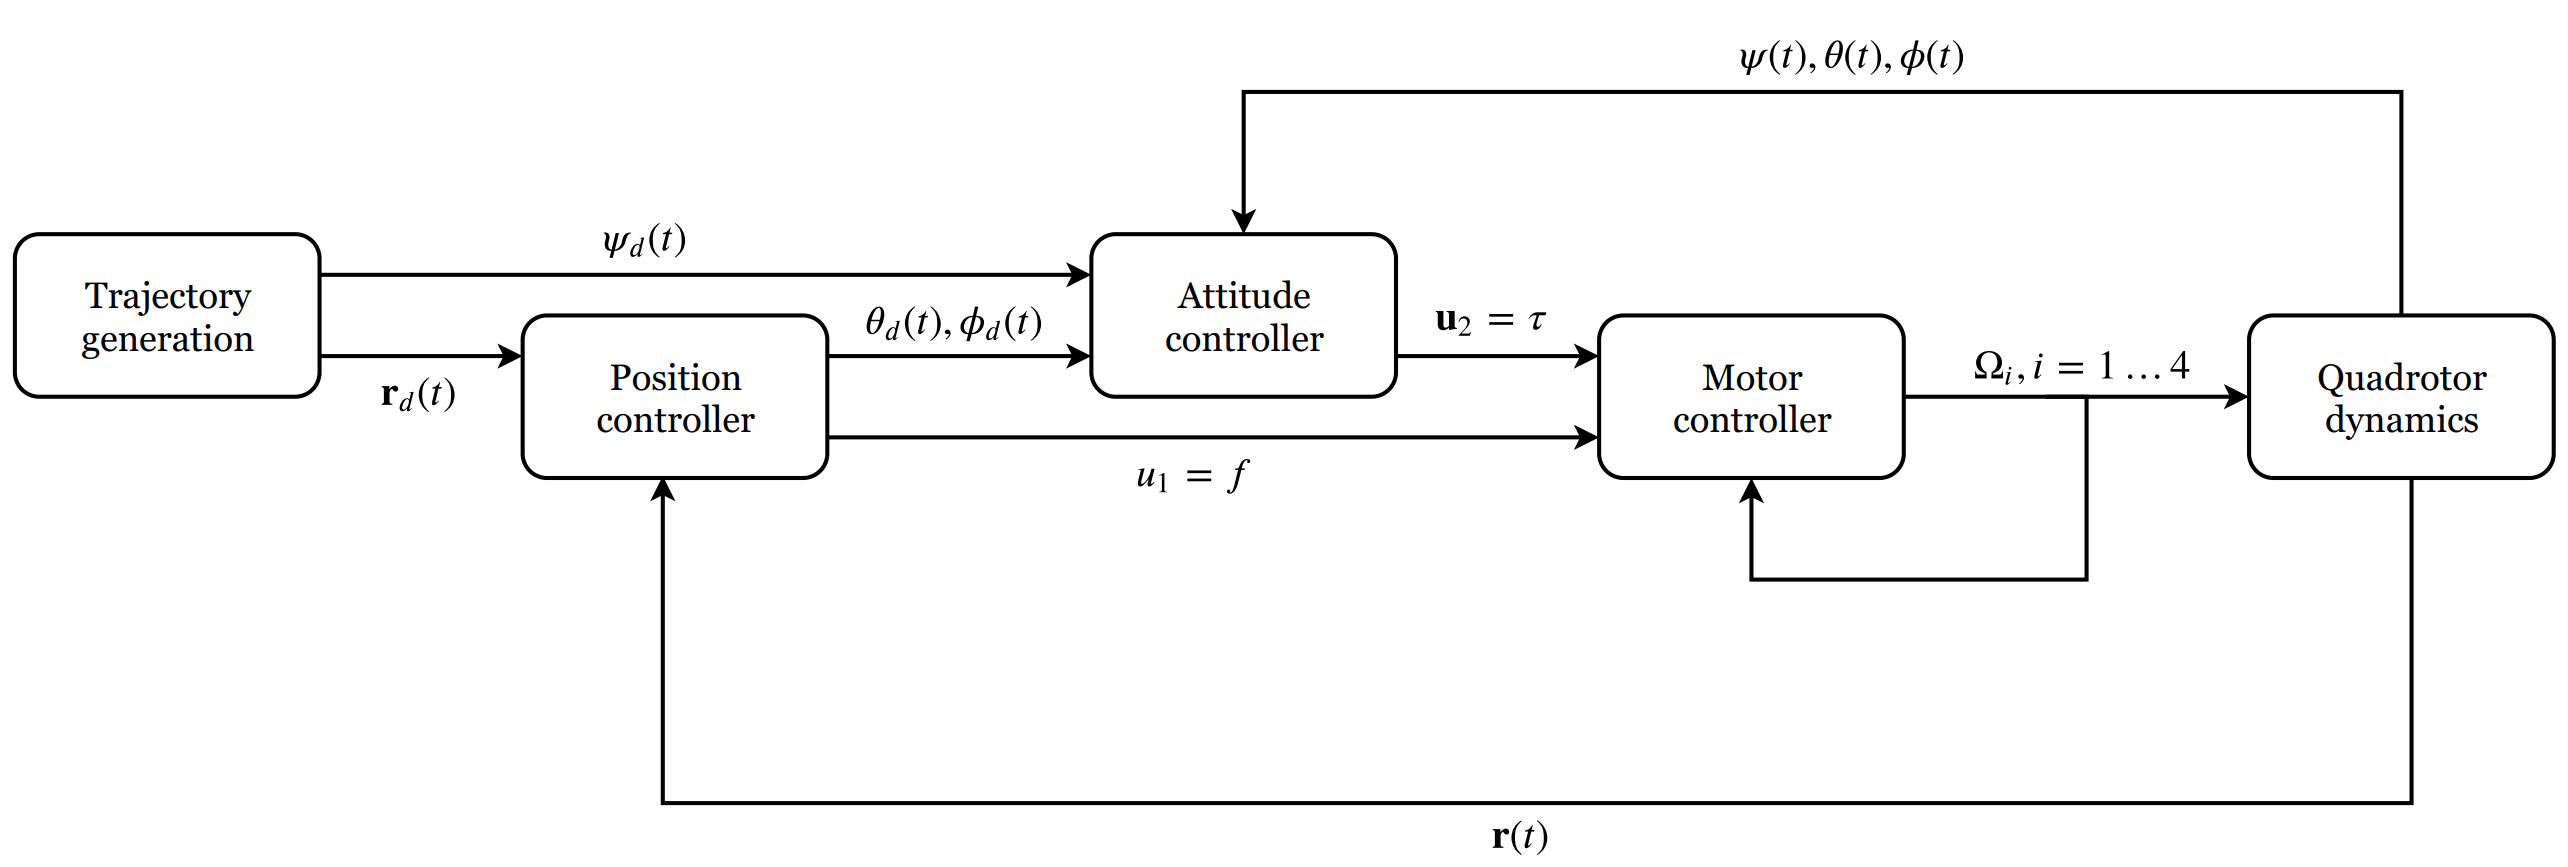
\includegraphics[width=0.8\textwidth]{Images/Control/General_control_architecture}
 \caption{General control architecture of a quadrotor.}
 \label{General_control_architecture}
 \end{figure}
 
 
 
 \newpage 
 \section{General Control Approaches}

\subsection{Method of Linearization}

By using extreme assumptions, it is feasible to apply linear control techniques in order to control a quadrotor (\cite{Sabatino2015}, \cite{BouabdallahNothSiegwart2018}). Particularly, this can be made by doing a linearization of the full dynamic model around an equilibrium point $\overline{\textbf{\textsc{x}}}$ and by using the assumption that the vehicle is only capable of oscillating lightly around the hover point.
It is very easy to observe that a feasible equilibrium is provided by a configuration where the center of mass is at a random position $\overline{\textbf{\textsc{r}}}$ and all the other elements of the state are set to zero. So, the nominal input $\bm{U} = \overline{\textbf{\textsc{U}}}$ to sustain such equilibrium can be assessed as the thrust that is required to compensate the gravity force:

\begin{equation}
\overline{\textbf{\textsc{u}}} = \begin{bmatrix}
f \\ 
\bm{\tau}\\
\end{bmatrix}=
\begin{bmatrix}
mg \\
\bm{0_{3 \times 1}} \\
\end{bmatrix}
\end{equation}

At this stage, the complete non-linear dynamics that have the form :

\begin{equation}
\dot{\textbf{\textsc{x}}}=\overline{\textbf{\textsc{f}}}(\overline{\textbf{\textsc{x}}},\overline{\textbf{\textsc{u}}})
\end{equation}

can now be linearized around the hover point $(\overline{\textbf{\textsc{x}}},\overline{\textbf{\textsc{u}}})$ as shown below.

\begin{equation}
\dot{\textbf{\textsc{x}}} = \begin{bmatrix}
\frac{\partial \textbf{\textsc{f}}(\textbf{\textsc{x}},\textbf{\textsc{u}})}{\partial \textbf{\textsc{x}}}
\end{bmatrix}_{(\bar{\textbf{\textsc{x}}},\bar{\textbf{\textsc{u}}})} \textbf{\textsc{x}}+ 
\begin{bmatrix}
\frac{\partial \textbf{\textsc{f}}(\textbf{\textsc{x}},\textbf{\textsc{u}})}{\partial \textbf{\textsc{x}}}
\end{bmatrix}_{(\bar{\textbf{\textsc{x}}},\bar{\textbf{\textsc{u}}})} \textbf{\textsc{u}} = \textbf{\textsc{A}}\textbf{\textsc{x}} + \textbf{\textsc{B}} \textbf{\textsc{u}}
\end{equation}

It can be demonstrated that both matrices $\textbf{\textsc{A}}$ and $\textbf{\textsc{B}}$ can be used to determine a linear system that is both controllable and observable \cite{Sabatino2015}. Thus, any control technique that is linear can now be used on the quadrotor in order to keep it areound a desired equilibrium point, such as optimal LQR/LQG \cite{Cowling2007,Minh2010} control or simple PD or PID controller \cite{Han2012,Altug2007}.



 \subsection{Internal Lyapunov Stability}
 
Before defining the \textit{Lyapunov Direct Method}, the notion of stability will be thoroughly defined first.

\subsubsection{Notions of Stability}
 For a general system without any control input
 
\begin{align}
 \dot{x}(t) &= f(x(t),0,t) \hspace{1in} (CT) \\
 \dot{x}(k+1) &= f(x(k),0,k) \hspace{1in} (DT),
\end{align}

 it is said that a point $\overline{x}$ is called an \textit{equilibrium point} from time $t_0$ for the continuous system (CT) if $f(\overline{x},0,t)=0,$ $\forall t \geq t_0$. Moreover, in the discrete time (DT) case, the point $\overline{x}$ is an equilibrium point from time $k_0$ if $f(\overline{x},0,k)=0,$ $\forall k \geq k_0$.
If the system begins from state $\overline{x}$ at time $t_0$ or $k_0$, then the system will stay there and will not change with time. It is possible for nonlinear system to have more than one equilibrium point (equilibria). There also exists another class of special solutions in the case of nonlinear systems, these solutions are called \textit{periodic} solution. However, it is outside the scope of this bibliography and interested readers are referred to \cite{Schmitt1972} for more in depth explanation. So, the focus will be on equilibria. It is desired to identify the \textit{stability} of the equilibria in some way. For instance, it is desired to know if, given some small perturbation to the system, the state would either come back to the equilibrium point, remain close to it in some sense, or it diverges.

The most useful notion of stability for an equilibrium point of a nonlinear system is provided by the definition below. Assuming that the equilibrium point is at the origin, because if $\overline{x} \neq 0$, a simple translation can be done to obtain a system that is equivalent with the equilibrium at the origin.

\paragraph{Asymptotic stability} A system is said to be \textit{asymptotically stable} about its own equilibrium point at the origin if the following two conditions are satisfied \cite{Dahleh2011}:

\begin{enumerate}
	\item For any $\epsilon > 0$, $\exists \delta_1 > 0$ such that if $\| x(t_0)\|<\delta_1$, then $\|x(t)\|<\epsilon, \forall t>t_0$.
	\item $\exists \delta_2$ such that if $\|x(t_0)\|<\delta_2$, then $x(t)\rightarrow 0$ at $t \rightarrow \infty$.
\end{enumerate}

For the first condition, it is required that the state trajectory should be restricted to a randomly small \textit{"ball"} that is centered at the equilibrium point and has a radius $\epsilon$, when released from aa \textit{arbitrary} initial condition in a ball that has an adequately small (yet positive) radius $\delta_1$. This is referred to as \textit{stability in the sense of Lyapunov} (i.s.L.). It is also possible to have stability in the sense of Lyapunov without having asymptotic stability, in that case, it is said that the equilibrium point is \textit{marginally stable}. Moreover, there also exist nonlinear systems that satisfy the second condition without being stable in the sense of Lyapunov. Moreover, an equilibrium point that is \textit{not} stable in the sense of Lyapunov is said to be \textit{unstable}.

\subsubsection{Lyapunov's Direct Method}

\paragraph{General Idea}

If the following continuous-time system is considered

\begin{equation} \label{Lyapunov_nonlinear_equation}
\dot{x}(t) = f(x(t))
\end{equation}
which has an equilibrium point at the origin (x=0).This system is called a time-invariant system because $f$ does not depend explicitly on the time t. In such a system, the stability analysis of the equilibrium point is in general a tedious task. This is because there is no way to write a simple formula which relates the trajectory to the initial state. The main idea of \textit{Lyapunov's direct method} is to establish properties of the equilibrium point (of the nonlinear system in general) by evaluating how a certain carefully chosen scalar function of the changes as the state of the system changes. (The term \textit{"direct"} is used to distinguish this method from the Lypunov's \textit{"indirect"} method, which tries to establish properties of the equilibrium point by assessing the behavior of the \textit{linearized} system at that point \cite{MELCHORAGUILAR2004175}.

As an example, a continuous and scalar function $V(x)$ that is equal to 0 at the origin and positive elsewhere is considered in some ball that is enclosing the origin. So, $V(0)=0$ and $V(x)>0$ when $x \neq 0$ in this ball. This $V(x)$ be considered as an \textit{"energy"} function. Also, let $\dot{V}(x)$ denote the time derivative of $V(x)$ throughout any trajectory of the system. In other words,  $\dot{V}(x)$ varies as $x(t)$ varies proportionally to equation (\ref{Lyapunov_nonlinear_equation}). If this derivative is negative in all the region (with the exclusion of the origin), then this means that the energy is decreasing with time in a strict manner. Moreover, since the lower bound of the energy is 0, then the energy must go to 0 with time. This means that all trajectories will converge to the origin (zero state). This idea is formalized below.




\newpage

\paragraph{Lyapunov Functions}

Assuming V is a continuous map from $\mathbb{R}^n$ to $\mathbb{R}$. $V(x)$ is called a \textit{locally positive definite} (lpd) function about x=0 if 

\begin{enumerate}
	\item $V(0)=0$.
	\item $V(x)>0$, $0<\|x\|<r$ for a given $r$.
\end{enumerate}

Also, the function is called locally \textit{positive semidefinite} (lpsd) id the strict inequality applied on the function in the second condition is changed to $V(x) \geq 0$. The function $V(x)$ is locally \textit{negative definite} (lnd) if $-V(x)$ is lpd. Moreover, $V(x)$ is locally \textit{negative semidefinite} (lnsd) if $-V(x)$ is lpsd. In order to graphically illustrate the locally positive definite function $V(x)$, it is useful to imaging having "contours" of constant $V$ that form (at least in a tiny region about the origin) a set of nested surfaces that are encircling the origin. An example is given in figure \ref{Lyapunov_figure} below. 


\begin{figure}[h]
\centering
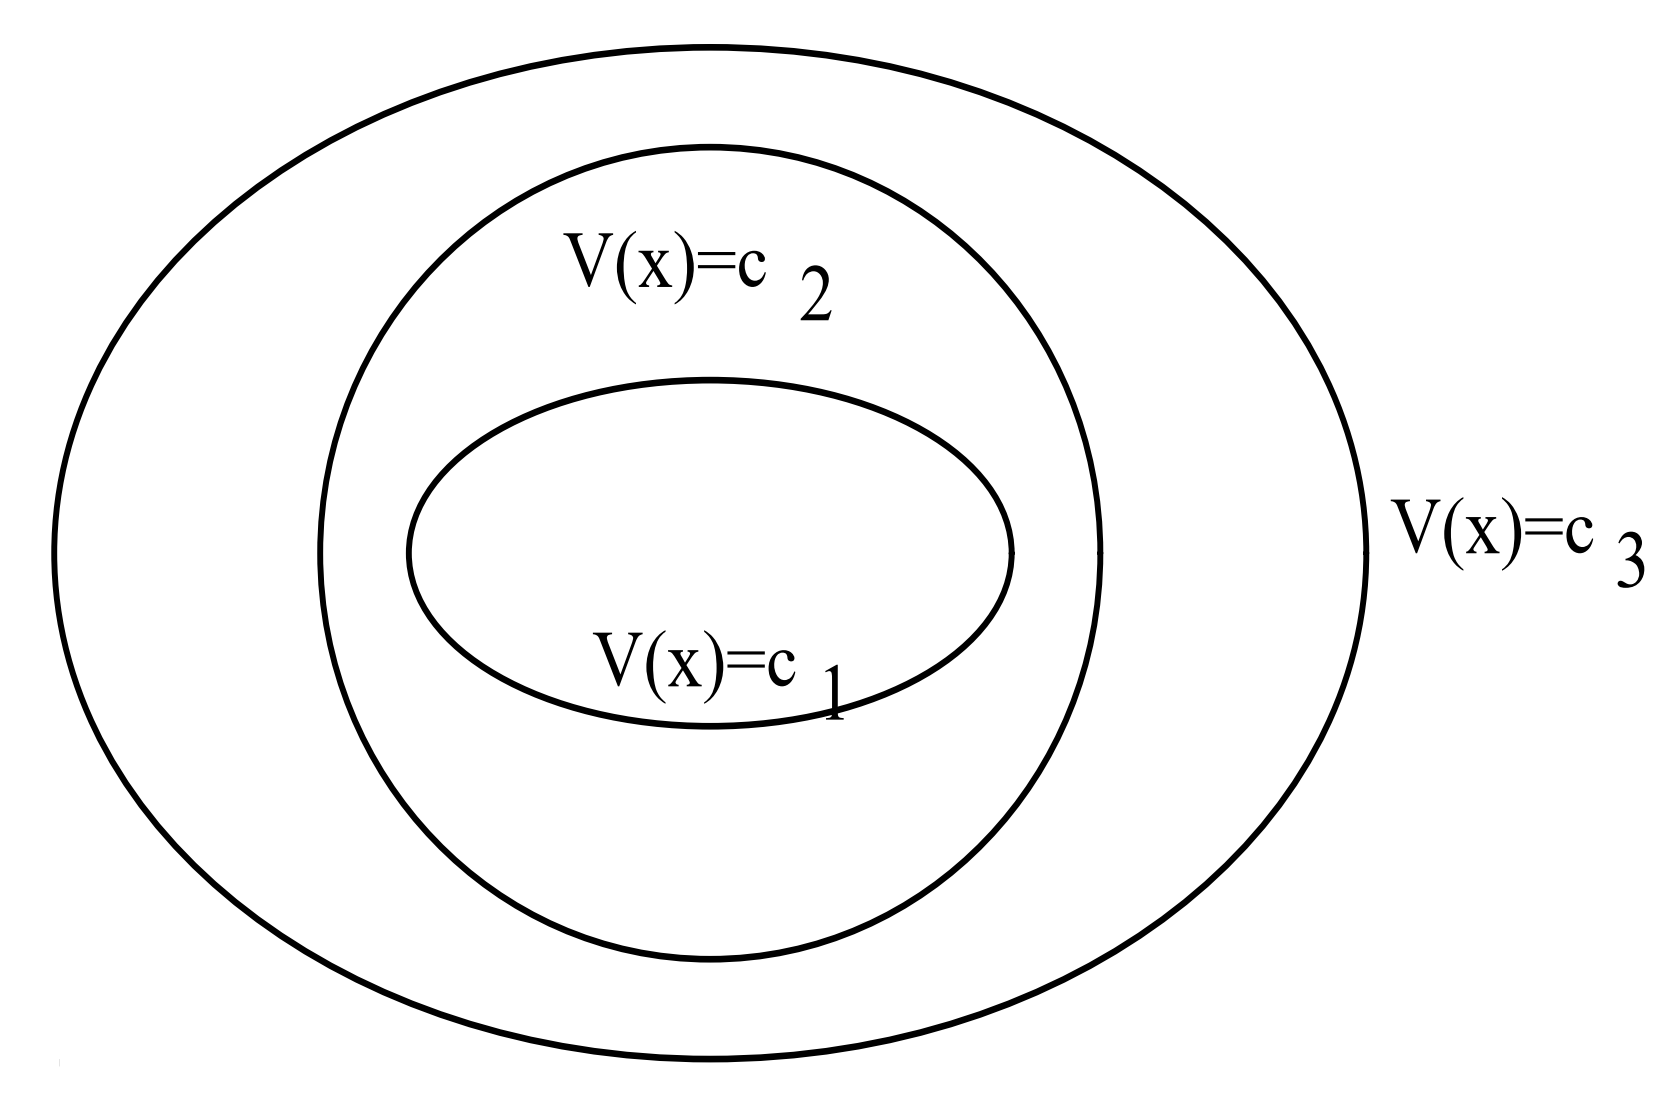
\includegraphics[width=0.6\textwidth]{Images/Control/Lyapunov_function}
\caption{Diffrenet values for a Lyapunov function, where $c_1<c_2<c_3$. \cite{Dahleh2011}}
\label{Lyapunov_figure}
\end{figure}

In the continuous time case, the focus in this bibliography will be restricted to $V(x)$ that has first partial derivatives that are continuous. (In the case of discrete time, only continuity will suffice, so differentiability is not required in that case.) The derivative of $V$ with respect to time \textit{along a trajectory of the system} \ref{Lyapunov_nonlinear_equation} is denoted as $\dot{V}(x(t))$. This derivative is expressed as follows:

\begin{equation}
\dot{V}(x(t)) = \frac{dV(x)}{dx}\dot{x} = \frac{dV(x)}{dx}f(x)
\end{equation}
where 
$\frac{dV(x)}{x}$ is the \textit{Jacobian} of $V$ with respect to $x$ which contain the partial derivative $V$ with respect to every component of $x$: $\frac{\partial V}{\partial x_i}$.

Moreover, assuming $V$ is a lpd function (a "candidate Lyapunov function"), and $(\dot{V})$ is the derivative along trajectories of the system of equation \ref{Lyapunov_nonlinear_equation}. Then,$V$ is called a \textit{Lyapunov function} of the system of equation \ref{Lyapunov_nonlinear_equation} if $\dot{V}$ is lnsd \cite{Dahleh2011}.


\paragraph{Lyapunov Theorem for Local Stability}

If a Lyapunov function for the system of equation (\ref{Lyapunov_nonlinear_equation}) exists, this means that $x=0$ is a stable equilibrium point in the sense of Lyapunov. Moreover, if $\dot{V}<0$, $0<\|x\|<r_1$, for some $r_1$, in other words, if $\dot{V}$ is lnd, this means that $x=0$ is an equilibrium point that is asymptotically stable\cite{Dahleh2011}.




\begin{comment}
In order to demonstrate this, the stability in the sense of Lyapunov must first be proven. Assuming that $\epsilon>0$ is given. Then a $\delta>0$ must be found such that for all $\|x(0)\|<\delta$, it follows that $\|x(t)\|<\epsilon$, $\forall t>0$. 

\newpage

The figure \ref{Lyapunov_proof_a} below shows the constructions of the proof.

\begin{figure}[h]
\centering
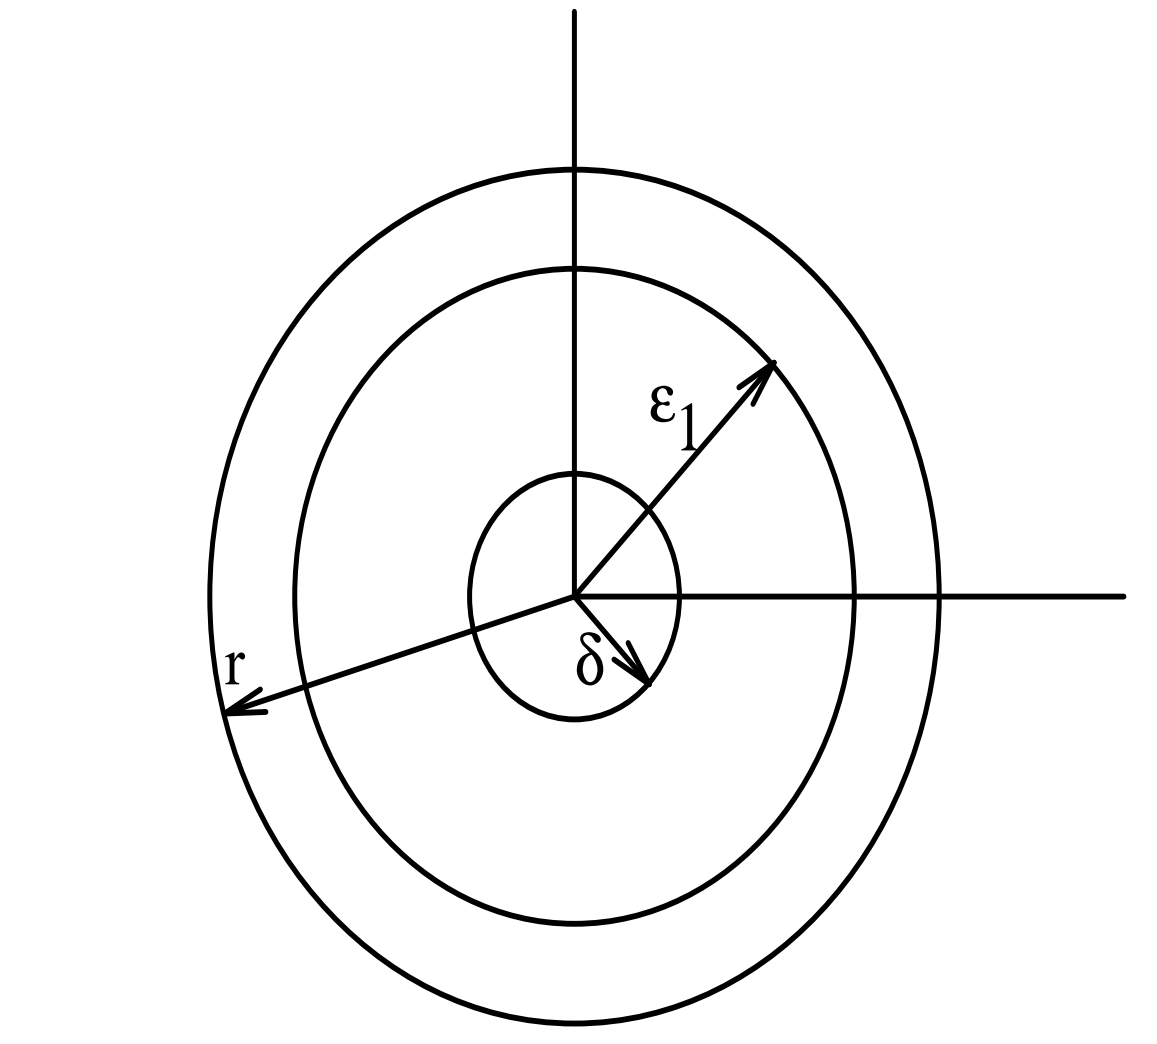
\includegraphics[width=0.6\textwidth]{Images/Control/Proof}
\caption{Representation of the neighborhoods used for the proof \cite{Dahleh2011}.}
\label{Lyapunov_proof_a}
\end{figure}

Let $\epsilon_1 = \min(\epsilon,r)$. And, assuming:

\begin{equation}
m = \min_{\|x\|=\epsilon_1} V(x)
\end{equation}

Since $V(x)$ is continuous, then $m$ is positive and well defined. Then a value $\delta$ can be chosen with $0<\delta<\epsilon_1$ such that for all $\|x\|<\delta$
, $V(x)<m$. 

\end{comment}



\paragraph{Lyapunov Theorem of Global Asymptotic Stability}

The region in the state space for which the earlier results hold is determined by the region over which $V(x)$ represents a Lyapunov function. It is interesting to determine the "basin of attraction" of an equilibrium point that is asymptotically stable. In other words, the basin of attraction is the set of initial conditions whose following trajectories conclude at the equilibrium point. Thus, an equilibrium point is \textit{"globally asymptotically stable"} ( also called asymptotically stable "in the large") if its basin of attraction is the entire state space.\\

\noindent
If a function $V(x)$ has the following criteria below, 

\begin{enumerate}
	\item $V(x)$ is positive definite throughout the state-space.
	\item $V(x)$ also has the added property that $|V(x)| \rightarrow \infty$ as $\|x\| \rightarrow \infty$.
	\item The derivative of $V$ (in other words $\dot{V}$) is negative definite throughout the state-space.
\end{enumerate}
Then, the equilibrium point at the origin is globally asymptotically stable \cite{Dahleh2011}.

\paragraph{Discrete-Time Systems}

Fundamentally identical results hold for the system

\begin{equation}
x(k+1) = f(x(k))
\end{equation}

provided that $\dot{V}$ is represented as

\begin{equation*}
\dot{V}(x) \triangleq V(f(x)) - V(x),
\end{equation*}

in other words as 

\begin{equation*}
V(\text{next state}) - V(\text{present state})
\end{equation*}


 \subsection{Model Predictive Control}
 \subsubsection{General Idea}\label{MPC_General_Idea}
 
 There exist "open-loop" methods \cite{Kirillova2000} in which the control input sequence $\textbf{\textsc{u}}(t)$ is designed using a model of the system and a set of constraints. However, the problem with this approach is that modeling error and noise are not taken into consideration. So, these inputs will not necessarily generate the desired response from the system. Because of that, a "closed-loop" strategy is required in order to cancel out these errors. So, an approach that can be used is called \textit{"Model Predictive Control"} (MPC). This approach is also known as \textit{"receding horizon control"} \cite{How2008} since the \textit{"prediction horizon"} (finite horizon) shifts forward by one time step after the current optimization problem is solved . In short, MPC is a \textit{feedback control} algorithm which uses a model of the system to predict the future outputs of the system and it solves an optimization problem on-line in order to select an optimal control.

\newpage 
 
 \paragraph{Basic strategy}

The basic strategy of MPC is following:


\begin{itemize}
	\item At time instant $k$, the system model and an optimizer will be used in order to design a sequence of control inputs
	
	$$ \textbf{\textsc{u}}(k|k), \textbf{\textsc{u}}(k+1|k), \textbf{\textsc{u}}(k+2|k), \textbf{\textsc{u}}(k+3|k),...,\textbf{\textsc{u}}(k+N|k) $$
	
	starting from the current state $\textbf{\textsc{x}}(k)$ over a prediction horizon $N$.
	\item Only the first step of the sequence of control inputs will be applied on the system.
	\item The processes above are then iterated for time $(k+1)$ at state $\textbf{\textsc{x}}(k+1)$. 
\end{itemize}
 
 
 \begin{figure}[h]
 \centering
 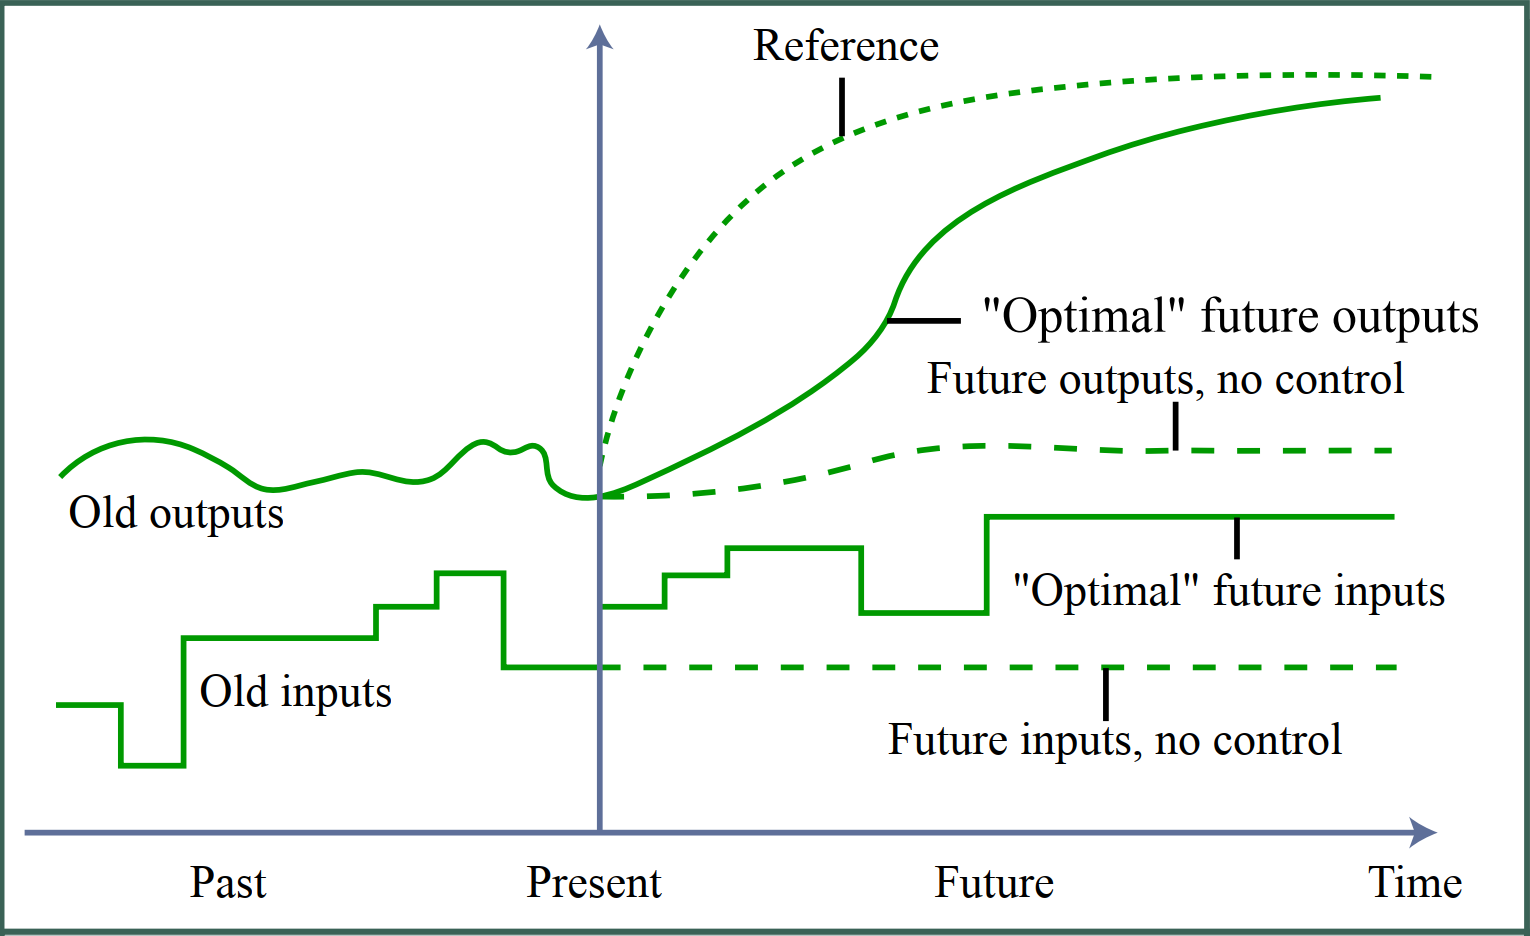
\includegraphics[width=0.6\textwidth]{Images/control/MPC_general_idea}
 \caption{Basic idea of MPC \cite{How2008}.}
 \label{MPC_basic_idea}
\end{figure}  
 
\noindent It should be noted that the control algorithm of MPC is based on numerically solving an optimization problem at each time step. In general, it is a constrained optimization.
 
 \paragraph{Advantages and drawbacks of MPC} There are several advantages when using MPC: 
 
 \begin{itemize}
 	\item MPC is able to control multi-input multi-output (MIMO) systems which might have interactions between their inputs and outputs
 	\item MPC explicitly accounts for the constraints that are imposed on the system. So, it does not just design a controller to keep the system away from the constraints.
 	\item MPC can easily handle nonlinear dynamics and time-varying plant dynamics, because the controller is explicitly a function of the model of the system which can be modified in real-time.
 \end{itemize}

\noindent The main drawback of MPC is that it usually requires a powerful and fast processor with a large memory in order to properly solve the problem at hand, because it solves an optimization problem at each time instant.
 
\noindent There have been many commercial applications of MPC starting from the early 1970s in the process industry. The table \ref{table_MPC} below shows the different companies that have used MPC in different industries in 2014.
 
\newpage

\begin{table}[h]
\setlength{\tabcolsep}{15pt} % Default value: 6pt
\renewcommand{\arraystretch}{1} % Default value: 1
 \caption{MPC applications in different industries in 2014.\cite{Kozak2014}}
 \label{table_MPC}
\begin{tabular}{l c c c c c r}
Application & Aspen & Honeywell & Adersa & CCI & Pavilion & Total \\
\hline
Refining & 950 & 300 & 290 & - & 15 & 1555 \\
Chemicals & 437 & 55 & 12 & 21 & 25 & 550 \\
Food & - & - & 48 & - & 14 & 62 \\
Pulp paper & 21 & 39 & - & - & 3 & 63 \\
Gas and air & 11 & 13 & - & 24 & - & 48 \\
Polymer & 5 & - & - & - & 22 & 27 \\
Utilities & 7 & 9 & - & 6 & - & 22 \\
Other & 39 & - & 51 & 6 & - & 96 \\
\hline 
\hline
Total & 1470 & 416 & 401 & 57 & 79 & 2423 \\
\end{tabular}
\end{table}

\noindent However, as computational power has increased throughout the years thanks to the advancement of technology, there has been a renewed curiosity in applying this control approach to systems with fast dynamics for which the computational complexity is significantly larger when compared to the industrial applications for which computational complexity was not a concern (since MPC was applied on systems with slow dynamics in that case).
 
\subsubsection{Design Parameters}
The different parameters that can be tuned in a MPC controller are the following:

\begin{itemize}
	\item The sample time $T_s$.
	\item The prediction horizon $N$.
	\item The control horizon $m$.
	\item The constraints.
	\item The weights.
\end{itemize}

\noindent Choosing the proper values for the parameters stated above is very important since they affect the performance of the controller and the computational complexity of the MPC algorithm.

\paragraph{Sample Time $T_s$} 

The sample time determine the rate at which the controller executes the control algorithm. \begin{itemize}
	\item If $T_s$ is too large, then when a disturbance occurs, the controller will be unable to react to the disturbance quick enough.
	\item If $T_s$ is too small, the controller will have much faster reaction times to disturbances and setpoint changes. However, this comes at the cost of an excessive computational load \cite{MathWorks2018}.
\end{itemize}

\noindent In order to find reasonable balance between controller performance and computational effort, the general recommendation is to have between 10\% and 25\% of the minimum desired close-loop response time \cite{MathWorks2018}.

\paragraph{Prediction horizon $N$} 

The prediction horizon $N$ (sometimes referred to with the variable $p$ \cite{MathWorks2018}, however, $N$ will be used instead for the remaining of this paper) is the number of predicted future time steps of the system. It shows how far the controller predicts into the future. Thus, a prediction horizon must be chosen in such a way that it covers the significant dynamics of the system. However, it should be noted that a large prediction horizon should not be selected, since unexpected phenomenons could occur that may affect the dynamics system, which will cause a waste of computational power. The general recommendation is to increase $N$ until additional increases will have little impact on the performance. The maximum $N$ is the number of control intervals needed for the open-loop step response of the system to become infinite. However, having $N>50$ is hardly ever required unless $T_s$ is very small \cite{MathWorks2018}.

\paragraph{Control horizon m}

The control horizon is the set of future actions which will lead to the predicted plant output. It represent the number of control moves until time step $m$. After the first $m$ steps, the remain inputs will remain constant as shown in figure \ref{MPC_basic_idea} for the \textit{"Optimal" future inputs}. Moreover, each control input element in the control horizon is a free variable that will be computed by the optimizer. Thus, the smaller the control horizon, the fewer the computations. However, setting $m=1$ may not give the best possible output for the system. And, similarly to the prediction horizon, if the control horizon is increased, this will lead to better predictions at the cost of increasing the computational complexity. Moreover, the general recommendation for the control horizon is to keep it much smaller than the prediction horizon \cite{MathWorks2018},because:

\begin{itemize}
	\item A smaller control horizon $m$ will lead to less variables to optimize in the QP that will be solved at each control input interval. This will encourage quicker computation times.
	\item If delays are considered, then having $m<N$ is mandatory. If not, some control input elements within the control horizon  may not have any effect on the plant outputs before the prediction horizon ends, which will lead to a QP Hessian matrix which is singular. 
	\item Having a small value for $m$ encourages having an internally stable controller. However, this is not guaranteed.
\end{itemize}

\paragraph{Constraints} A model predictive controller can integrate constraints on the inputs, the rate of change of the inputs and the outputs. In addition, the constraints can be \textit{"soft"} constraints or \textit{"hard"} constraints. However, it should be noted that hard constraints cannot be violated. In addition, applying hard constraints on both the inputs and outputs at the same time may cause conflict to occur between the constraints, which may lead to an unfeasible solution. Moreover, the general recommendation is to used soft constraints on the outputs and to avoid having hard constraints on both the inputs and the rate of change of the inputs \cite{MathWorks2018b}.

\paragraph{Weights} Model Predictive Control could have many goals. One goal could be to have the outputs converge to their set-points as fast as possible. Another goal can be to have smooth control inputs in order to avoid aggressive control maneuvers. So, in order to achieve a balanced performance between these two competing goals, the input rates and the outs can be weighted relative to each other. It is also possible to adjust relative weights within the input rates and the outputs \cite{MathWorks2018c}.



\newpage
\subsubsection{Basic formulation} 

For a given set of plant dynamics which is first assumed to be linear:

\begin{equation}
\begin{cases}
\textbf{\textsc{x}}(k+1) = A\textbf{\textsc{x}}(k) + B \textbf{\textsc{u}}(k) \\
\textbf{\textsc{z}}(k) = C \textbf{\textsc{x}}(k)\\
\end{cases}
\end{equation}

\noindent and a cost function as follows: 

\begin{equation}
J = \sum_{j=0}^{N} \{ \|\textbf{\textsc{z}}(k+j|k)\|_{R_{zz}} + \|\textbf{\textsc{u}}(k+j|k)\|_{R_{uu}} \} + F \textbf{\textsc{x}}(k+N|k))
\end{equation}

 
\noindent With: 
 
 \begin{itemize}
 	\item $\|\textbf{\textsc{z}}(k+j|k)\|_{R_{zz}}$ is the weighted $L^2$ norm of the state, so it is expressed as follows:

 \begin{equation*}
 \|\textbf{\textsc{z}}(k+j|k)\|_{R_{zz}} = \textbf{\textsc{z}}(k+j|k)^{\intercal}R_{zz}\textbf{\textsc{z}}(k+j|k)
\end{equation*}   	
 	
	\item  	$\|\textbf{\textsc{u}}(k+j|k)\|_{R_{uu}}$ is the weighted $L^2$ norm of the control input sequence, so it is expressed as follows:
	
\begin{equation*}
 \|\textbf{\textsc{z}}(k+j|k)\|_{R_{zz}} = \textbf{\textsc{z}}(k+j|k)^{\intercal}R_{zz}\textbf{\textsc{z}}(k+j|k)
\end{equation*}  

	\item $F \textbf{\textsc{x}}(k+N|k))$ is a terminal cost function.
 	
\end{itemize}  
 
It should be noted that if  $N \rightarrow \infty$, and there are no additional constraints on  $\textbf{\textsc{z}}$ or $\textbf{\textsc{u}}$, then the problem falls back to the discrete LQR problem \cite{Kostova2013}. Moreover, when limits are added on 
  $\textbf{\textsc{x}}$ or $\textbf{\textsc{u}}$, then the general solution cannot be found anymore in analytical form, and it has to be solved numerically.

Moreover, solving for a very long sequence of control input is useless if the model used for the computations is expected to be erroneous or there are distrubances applied on the system, since only the first element the optimized control sequence only will be implemented. This is why MPC is designed by using a small $N$. 
  
  \paragraph{Typical problem statement}
  
  For a finite $N$ and $F=0$ the problem can be expressed as follows: 
  
\begin{mini}|s|
{u}{ J = \sum_{j=0}^{N}{  \{ \|\textbf{\textsc{z}}(k+j|k)\|_{R_{zz}} + \|\textbf{\textsc{u}}(k+j|k)\|_{R_{uu}} \} }}
{}{}
\addConstraint{ \textbf{\textsc{x}}(k+j+1|k) = A\textbf{\textsc{x}}(k+j|k) + B \textbf{\textsc{u}}(k+j|k) }
\addConstraint{ \textbf{\textsc{x}}(k|k) \equiv \textbf{\textsc{x}}(k) }
\addConstraint{\textbf{\textsc{z}}(k) = C \textbf{\textsc{x}}(k+j|k)}
\addConstraint{|\textbf{\textsc{u}}(k+j|k)| \leq u_m}
{}
\label{optim_problem}
\end{mini}

 \newpage  
  
  
  \noindent The problem statement in (\ref{optim_problem}) can be converted into a more standard optimization problem as follows:
  

  

  \begin{align*}
    	\textbf{\textsc{z}}(k|k) &= C \textbf{\textsc{x}}(k|k)\\
    	\vspace{1cm}\\
  	\textbf{\textsc{z}}(k+1|k) &= C \textbf{\textsc{x}}(k+1|k) = C (A\textbf{\textsc{x}}(k|k) + B\textbf{\textsc{u}}(k|k))\\
  	&=  C A\textbf{\textsc{x}}(k|k) + CB\textbf{\textsc{u}}(k|k)\\
  	\vspace{1cm}\\
  	\textbf{\textsc{z}}(k+2|k) &= C \textbf{\textsc{x}}(k+2|k) \\
  	&= C(A\textbf{\textsc{x}}(k+1|k) + B \textbf{\textsc{u}}(k+1|k)) \\
  	&= C A(A \textbf{\textsc{x}}(k|k) + B   	\textbf{\textsc{u}}(k|k)) + C B \textbf{\textsc{u}}(k+1|k)\\
  	&= C A^2 \textbf{\textsc{x}}(k|k) + CAB \textbf{\textsc{u}}(k|k) + CB \textbf{\textsc{u}}(k+1|k) \\
  	&\text{\hspace{0.2cm}}\vdots \\
  	 \textbf{\textsc{z}}(k+N|k) &=  C A^N \textbf{\textsc{x}}(k|k) + CA^{N-1}B\textbf{\textsc{u}}(k|k) + \ldots\\
  	 &\text{\hspace{0.5cm}} + CB\textbf{\textsc{u}}(k+(N-1)|k)\\	
  \end{align*}

 \noindent The equations above can then be grouped as follows:
 
 \begin{multline*}
 \begin{bmatrix}
 \textbf{\textsc{z}}(k|k) \\
 \textbf{\textsc{z}}(k+1|k)\\
 \textbf{\textsc{z}}(k+2|k)\\
 \vdots \\
 \textbf{\textsc{z}}(k+N|k)\\
 \end{bmatrix} = 
 \begin{bmatrix}
 C\\
 CA\\
 CA^2\\
 \vdots\\
 CA^N \\
 \end{bmatrix} \textbf{\textsc{x}}(k|k) \\
 + \begin{bmatrix}
 0 && 0 && 0 && \ldots && 0\\
 CB && 0 && 0 && && 0 \\
 CAB && CB && 0 && && 0 \\
 \vdots\\ 
 CA^{N-1}B && CA^{N-2}B && CA^{N-3}B && \ldots && CB \\
 \end{bmatrix}
 \begin{bmatrix}
 \textbf{\textsc{u}}(k|k)\\
 \textbf{\textsc{u}}(k+1|k)\\
 \vdots\\
 \textbf{\textsc{u}}(k+N-1|k)\\
 \end{bmatrix}
 \end{multline*}

\noindent Now $Z(k)$ and $U(k)$ can be defined as follows:

\begin{equation*}
Z(k) \equiv \begin{bmatrix}
\textbf{\textsc{z}}(k|k)\\
\vdots \\
\textbf{\textsc{z}}(k+N|k)\\
\end{bmatrix} 
\text{\hspace{1cm} , \hspace{1cm}}
U(k) \equiv \begin{bmatrix}
\textbf{\textsc{u}}(k|k)\\
\vdots \\
\textbf{\textsc{u}}(k+N-1|k)\\
\end{bmatrix} 
\end{equation*}  
  

\noindent It should be noted that:

\begin{equation*}
	\sum_{j=0}^{N}\textbf{\textsc{z}}(k+j|k)^{\intercal} R_{zz}\textbf{\textsc{z}}(k+j|k) = Z(k)^{\intercal}W_1Z(k)
\end{equation*}  
with $W_1$ denoting the weighting matrix.

\newpage

 \noindent Thus, the elements of the cost function in (\ref{optim_problem}) can now be expressed as follows:
  

  \begin{align}
  	Z(k)^{\intercal}W_1Z(k) + U(k)^{\intercal}W_2U(k) &=(G\textbf{\textsc{x}}(k) + HU(k))^{\intercal}W_1(G\textbf{\textsc{x}}(k) +HU(k)) + U(k)^{\intercal}W_2U(k) \nonumber \\
  &= \textbf{\textsc{x}}(k)^{\intercal}H_1\textbf{\textsc{x}}(k) + H_2^{\intercal} U(k) + \frac{1}{2}U(k)^{\intercal}H_3U(k)
  \end{align}
  
  With
  
  \begin{equation*}
  H_1 = G^{\intercal} W_1 G, \text{\hspace{0.5cm}} H_2 = 2(\textbf{\textsc{x}}(k)^{\intercal}G^{\intercal}W_1H), \text{\hspace{0.5cm}} H_3 = 2(H^{\intercal} W_1 H + W_2)
  \end{equation*}

\noindent Since the term $\textbf{\textsc{x}}(k)^{\intercal} H_1 \textbf{\textsc{x}}(k)$ does not contain the component to be minimized $U(k)$, this means that it will be constant throughout the optimization process. As a result, it can be omitted.
Finally, the MPC problem can be re-written as:

 \begin{mini}|s|
{\textsc{U}(k)}{ \tilde{J} = H_2^{\intercal} U(k) + \frac{1}{2}U(k) H_3 U(k) }
{}{}
\addConstraint{\begin{bmatrix}
I_N\\
-I_N\\
\end{bmatrix}U(k) \leq u_m}
{}
\label{MPC_problem}
\end{mini}
  
 \noindent Thus, the MPC problem has been transformed to the form of a quadratic program for which there exists various efficient tools to solve the problem. 
  



\subsubsection{MPC Observations} 

The current form of (\ref{MPC_problem}) assumes that the full state of the system is available. Moreover, a state estimator can also be used. In addition, the corresponding control is also assumed to be sensed and applied immediately on the system, this is usually a safe and reasonable assumption for most control systems. However, given that the optimization problem will be solved at each time step, then there is a possibility that accounting for this computation delay could be mandatory.

\paragraph{Case of no imposed constraints} 
If there are no active constraints on \ref{MPC_problem}, then the solution of the QP becomes

\begin{equation}
U(k) = - H_3^{-1}H_2
\end{equation}
which can be expressed as follows:

  \begin{align}
  	u(k|k) &= - \begin{bmatrix}
  	1 && 0 && \ldots && 0\\
  	\end{bmatrix}
  	(H^{\intercal} W_1 H + W_2)^{-1} H^{\intercal} W_1 G \textbf{\textsc{x}}(k) \\
  	&= -K \textbf{\textsc{x}}(k)
  \end{align}
which is nothing else but a state feedback controller.


\paragraph{Stability of MPC}

The stability of MPC greatly depends on the terminal cost and terminal constraints \cite{MAYNE2000789}. On the other hand, a classic result \cite{BEMPORAD19942013} states that if a Model Predictive Control algorithm was applied on a linear system with constraints, and assuming there exists terminal constraints: 

\begin{itemize}
	\item $\textbf{\textsc{x}}(k+N|k)=0$ for the predicted state $\textbf{\textsc{x}}$.
	\item $\textbf{\textsc{u}}(k+N|k)=0$ for the computed future control input $\textbf{\textsc{u}}$
\end{itemize}
And, if the optimization problem is realizable at time step $k$, then $\textbf{\textsc{x}}=0$ is stable.

\newpage


\subsubsection{Different MPC Methods}
The MPC methods that are mainly used are the following:

\begin{itemize}
	\item Linear time-invariant MPC.
	\item Adaptive MPC.
	\item Gain-Scheduled MPC.
	\item Non-linear MPC.
\end{itemize} 

\noindent The method to be used is chosen based on the complexity of the system at hand and on the required goals to be reached. 

\paragraph{In case of linear systems} The method to be used is called Linear time-invariant MPC. The constraints must be linear and the cost function must be quadratic. These characteristics will result in a convex optimization problem \cite{ZEMAN2003325} which has a global optimum. An example of a convex function is shown in figure \ref{convex_function} below.

\begin{figure}[h]
\centering
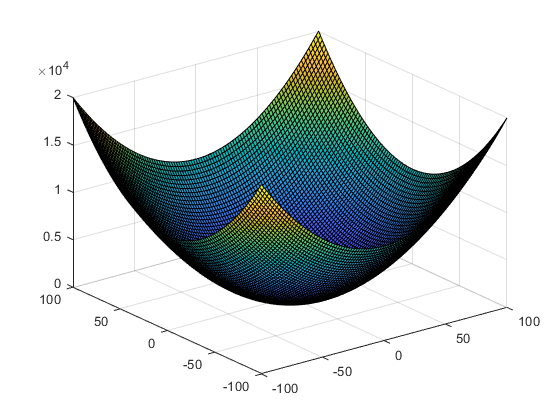
\includegraphics[width=0.6\textwidth]{Images/Control/MPC_Convex_Equation}
\caption{Representation of a convex function plotted using MATLAB.}
\label{convex_function}
\end{figure}

\paragraph{In case of a nonlinear systems} If the system is linearizable, then both Adaptive MPC and Gain-Scheduled MPC can be used in this case. But the constraints are still linear and the cost function is still quadratic. In this case, the nonlinear function can be linearized around an operating point, which will result in a linear function that approximates the nonlinear system well near the operating point. However, it should be noted that the linear function will not work well outside the operating region. This is why it is interesting to find multiple linearized models, with each model representing the nonlinear function well around it's operating point.



\begin{figure}[h]
\centering
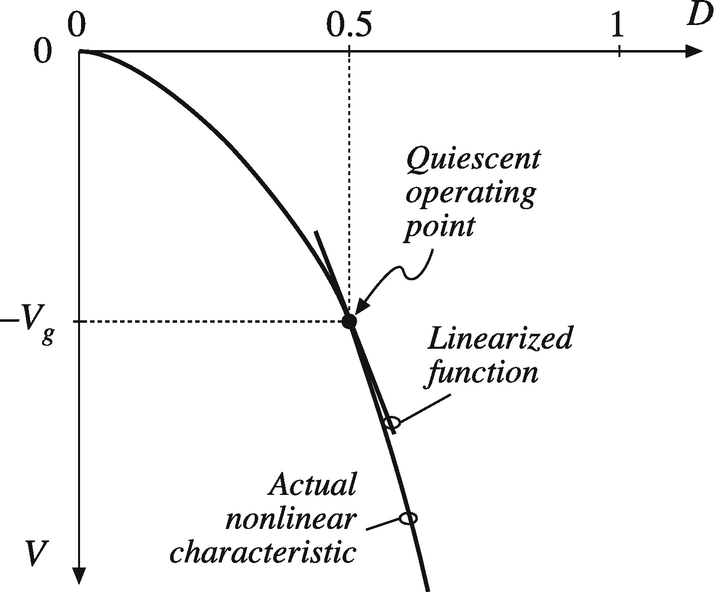
\includegraphics[width=0.45\textwidth]{Images/Control/linearization}
\caption{Example of the linearization of a nonlinear function around an operating point \cite{Erickson2020}.}
\label{nonlinear_function_linearization}
\label{non_convex_function}
\end{figure}



\paragraph{Adaptive MPC} In this case, a linear model is computed on-line as the operating conditions change. And, the internal plant model used by the MPC is updated with the corresponding linear model at each time step. Moreover, it should be noted that the optimization problem remains the same across different operating points. In other words, the number of elements in the state and the constraints remain the same across different operating conditions \cite{Bujarbaruah2018}.

\paragraph{Gain-Scheduled MPC} In this case, linearization of the nonlinear model is done offline at the operating points of interest. Then, a linear MPC controller is designed for each operating point. However, it should be noted that unlike Adaptive MPC, each controller is now independent from the other. In other words, the number of elements in the state and the constraints are different across different operating conditions.
It should also be noted that for this method, an algorithm must be designed to switch between the predefined MPC controllers for different operating conditions. Moreover, Gain-Scheduled MPC also uses more memory than Adaptive MPC \cite{7347864}.

\paragraph{Non-linear MPC} If the system is nonlinear and cannot be linearized, and both the constraints and the cost function are also nonlinear, then Nonlinear MPC can be used in that case. It is the most powerful method between all the different methods mentioned earlier, since it used the most accurate representation of the plant. Thus, predictions are more accurate. However, Nonlinear MPC is the most difficult method to solve in real-time. Because, in that case the problem becomes a non-convex optimization problem. Thus, the cost function may have many local minima, and finding the global minimum may be hard in that case. An example of a non-convex function is shown in figure \ref{nonconvex_function} below.


\begin{figure}[h]
\centering
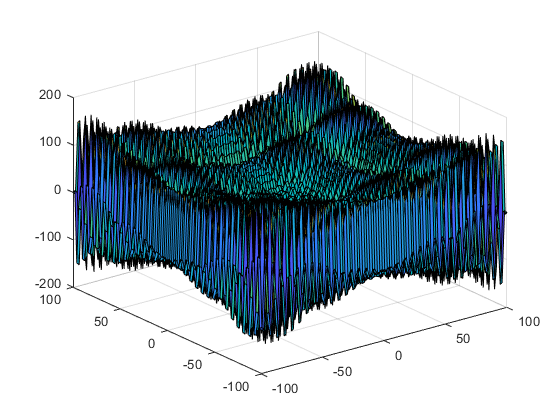
\includegraphics[width=0.6\textwidth]{Images/Control/MPC_Nonconvex_Equation_b}
\caption{Representation of a non-convex function plotted using MATLAB.}
\label{nonconvex_function}
\end{figure}

\newpage

\subsubsection{Strategies to Improve Computational Time}

As demonstrated in (\ref{MPC_problem}), an MPC problem is formulated as a QP problem that tries to minimize a quadratic cost function in general. Moreover, MPC computations become more complex as the number of state elements, the number of constraints and the MPC parameters increase. Moreover, as stated in section \ref{MPC_General_Idea}, if the MPC controller is running on applications with slow dynamics, then computational complexity is not a concern. However, if MPC is running on applications with fast dynamics, then the computational complexity becomes important. In addition, it is important to note that the matrices that are stored in the processor of the system for MPC computations grows with the increasing number of optimization variables. Thus, this will cause a memory problem. So, to reduce the complexity and computational time of MPC, the following methods can be used:

\paragraph{Order reduction techniques} They are used to discard states that do not contribute to the dynamics of the system \cite{4421358}. And, using order reduction techniques will also reduce the memory usage of the controller.

\begin{comment}
\paragraph{For applications with small $T_s$} In these cases, the performance of the MPC controller can be increased by \cite{bequette2003process}:
\begin{itemize}
	\item Shortening the prediction horizon.
	\item Shortening the control horizon.
	\item Reducing the number of constraints.
	\item Having lower precision operations and data representation.
\end{itemize} 
It should be noted that for applications with even smaller sample times, \textit{Explicit} MPC can be used.
\end{comment}

\paragraph{Explicit MPC} Instead of solving the optimization problem online for the current state, \textit{Explicit} MPC solves it offline for each value of the state \textbf{\textsc{x}} within a given range \cite{Bemporad2013}. Thus, for each state value within a given range, the Explicit MPC precomputes the optimal solution. And, this solution consists of linear functions that are piecewise affine and continuous is \textbf{\textsc{x}}. An example of Explicit MPC applied on a one-dimensional system is shown in figure \ref{Explicit_MPC_1D} below.

\begin{figure}[h]
\centering
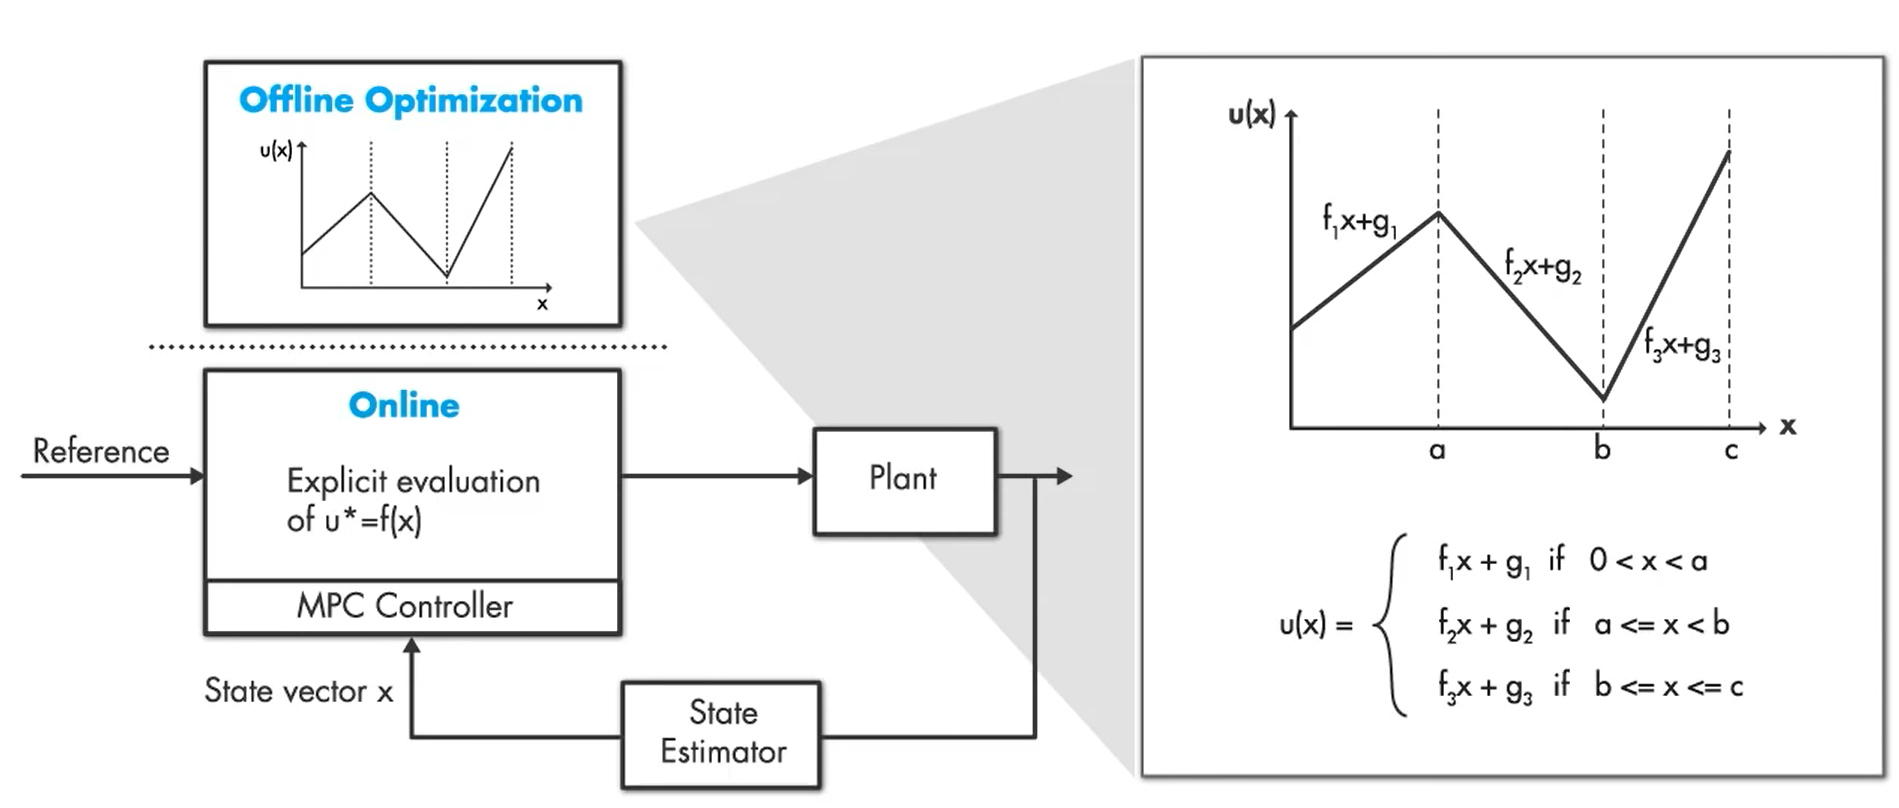
\includegraphics[width=0.9\textwidth]{Images/Control/Explicit_MPC_a}
\caption{Example of an Explicit MPC controller applied on a one-dimensional system \cite{MathWorks2018_new}.}
\label{Explicit_MPC_1D}
\end{figure}

\noindent As can be observed from figure \ref{Explicit_MPC_1D}, the constraints cut the solution space into different regions. And, each region maps into a unique solution.
Another example of an Explicit MPC applied on a two-dimensional system is shown in figure \ref{Explicit_MPC_2D} below. 

\newpage

\begin{figure}[h]
\centering
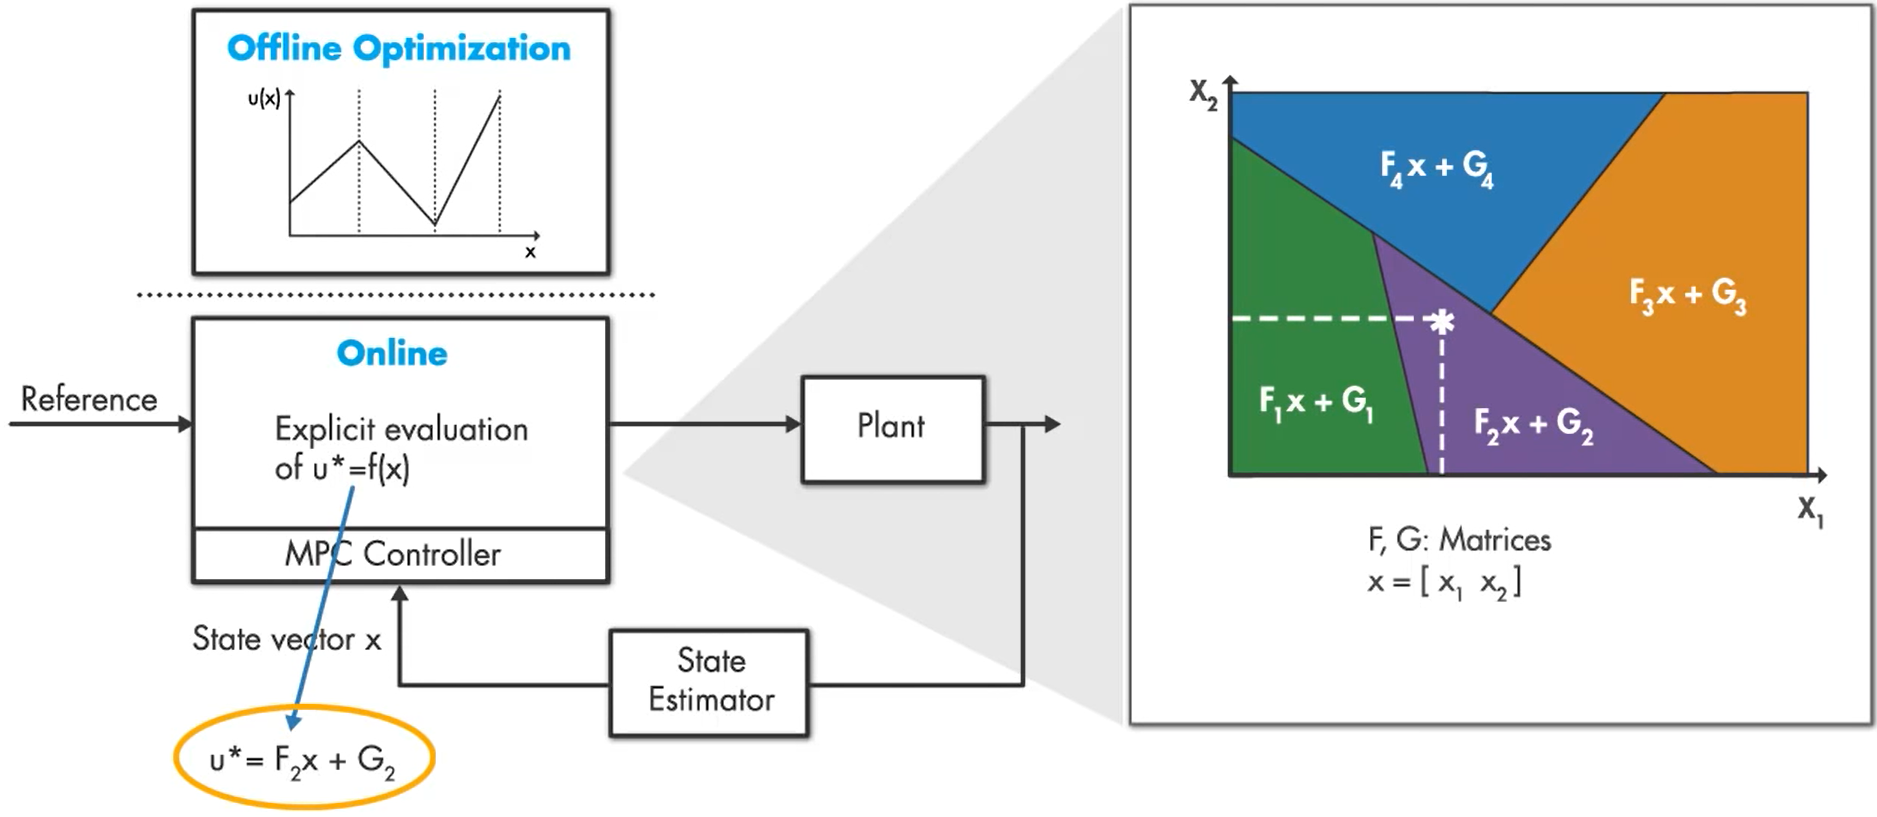
\includegraphics[width=0.9\textwidth]{Images/Control/Explicit_MPC_b}
\caption{Example of an Explicit MPC controller applied on a two-dimensional system \cite{MathWorks2018_new}.}
\label{Explicit_MPC_2D}
\end{figure}

\noindent As can be observed from figure \ref{Explicit_MPC_2D}, the Explicit MPC finds the  region that the current state lies in and evaluates the linear function that creates the current control input.

\noindent Thus, it can be concluded that if the iterative optimization process is reduced to linear function evaluations, then this will greatly simplify the online computations. However, if there is a large number of regions that the state can lie in, then searching for the current state region could sometimes be time consuming. Also, having many regions could cause memory problems for the processor. Thus, the number of regions can be reduced by merging some regions together. However, computed solution in that case is not optimal anymore \cite{Hovland2008}.

\paragraph{Suboptimal Solution}
It is another method to improve the computational time of the MPC controller. In a MPC problem, the optimal solution is very unpredictable and can drastically change between each time step. In addition, the computational time may exceed the sample time $T_s$. So, it is mandatory to make sure that a solution can be found within $T_s$ and that there still exists additional time for other tasks that need to be executed \cite{Gulez2014}. A simple example is provided in figure \ref{Suboptimal_solution_example} below where a maximum value for the iterations is determined and as an example, it is taken as 5. 


\begin{figure}[h]
\centering
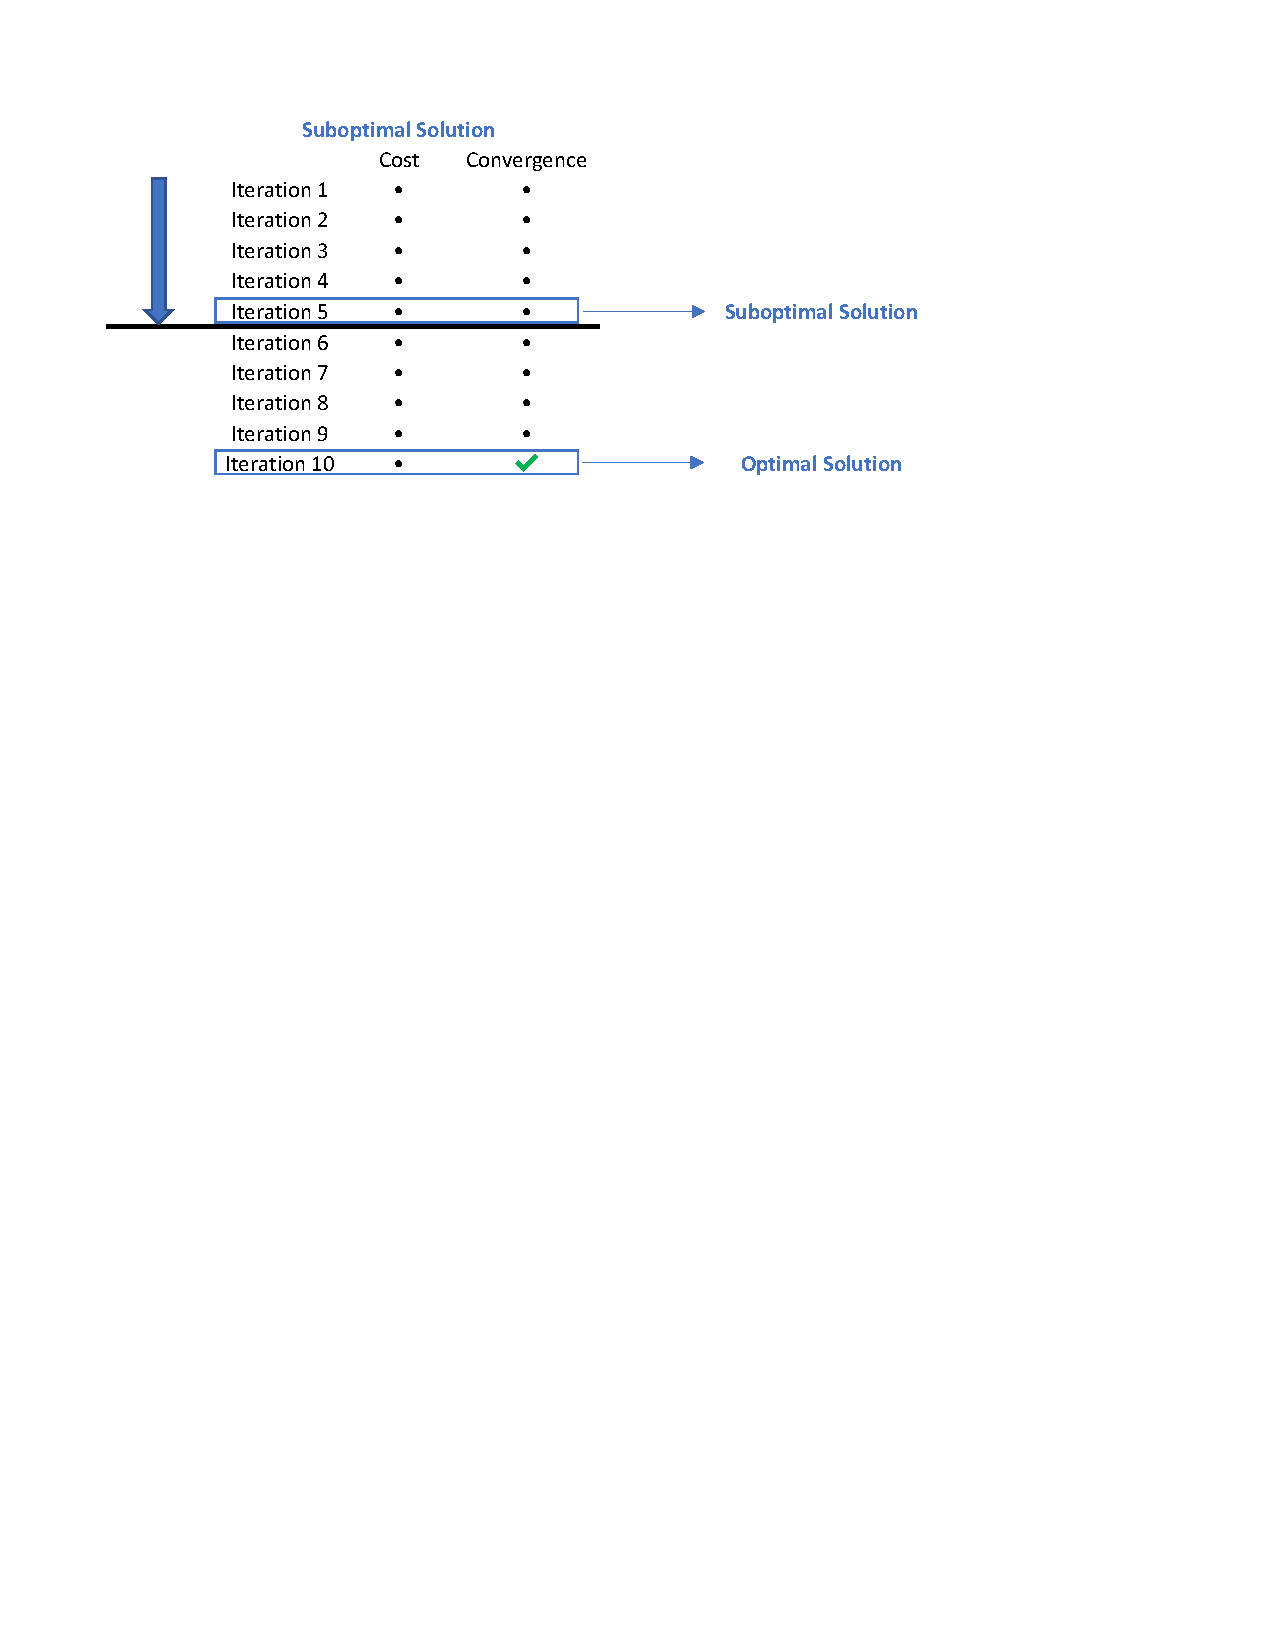
\includegraphics[width=0.8\textwidth]{Images/Control/Suboptimal_Solution.png}
\caption{Example showing how the suboptimal solution is found when the maximum number of iterations is set to 5.}
\label{Suboptimal_solution_example}
\end{figure}

\noindent As can be seen from figure \ref{Suboptimal_solution_example}, the optimal solution is reached in 10 iterations. However, the controller will stop at iteration 5 and take the suboptimal solution. Moreover, it is important to note that the suboptimal solution still satisfies all the constraints of the optimization problem. The only question that remain is how to determine the maximum number of iterations. This can be done by testing the algorithm on the hardware directly and identifying the execution time used by each iteration. Then, the maximum number of iterations is chosen such that the total execution time does not exceed the sample time of the controller.


  \subsubsection{Existing MPC toolboxes} Some of the available tools that allow to solve the MPC problem are listed below.
  
  \begin{itemize}
  	\item \textbf{Model Predictive Control Toolbox}\footnotemark : it is made by MathWorks (closed-source).
  	\item \textbf{MPCtools}\footnotemark : it is a free and open-source toolbox for MATLAB and Simultink that  permits to create and simulate basic MPC controllers by using linear state space models.
  	\item \textbf{do-mpc}\footnotemark : it is a free and comprehensive open-source toolbox for robust model predictive control (MPC) which is written in Python language.
  	\item \textbf{Control Toolbox}\footnotemark : it is an efficient library for control, estimation, optimization and motion planning in robotics problem that is written in C++ language.
  \end{itemize}
  

\footnotetext[1]{\url{https://www.mathworks.com/products/model-predictive-control.html}, accessed on 01/10/2021.}  

\footnotetext[2]{\url{http://www.control.lth.se/research/tools-and-software/mpctools/}, accessed on 01/10/2021.}  

\footnotetext[3]{\url{https://www.do-mpc.com/en/latest/}, accessed on 01/10/2021.}  

\footnotetext[4]{\url{https://github.com/ethz-adrl/control-toolbox}, accessed on 01/10/2021.}  




 \newpage
 \subsection{Sliding mode control}
 
 
 
  \subsubsection{Main Principles}
 
 
 
Sliding mode control (SMC) is a control technique that is nonlinear presenting exceptional attributes of robustness,
accuracy, easy tuning and execution.
 
The aim of SMS systems is to drive the system states to a specific surface in the state space, called sliding surface. Upon
reaching the sliding surface, sliding mode control allows the states to remain on the close neighborhood of the sliding
surface. Therefore, the sliding mode control consists of a controller design with two parts. The first part includes the
design of a sliding surface in order for the sliding motion to fulfill design requirements. The second deals with selecting a
control law that makes the switching surface interesting with respect to the system state \cite{Utkin1997}.




There exists two main benefits of sliding mode control. Firstly, the behavior of the dynamics of the system can be changed
according to a specific selection of the sliding function. Secondly, the response of the closed loop system becomes completely
insensitive to some special uncertainties. This principle goes beyond bounded model parameter uncertainties, interference and non-linearity.

In a practical sense, SMC allows the control of nonlinear processes that are affected by external noise and heavy model uncertainties.



The most important principles of SMC are shown in the following significant references \cite{Utkin1997,DeCarlo1998,Hung1993}\\



Researchers have also studied the problems appearing in the practical execution of this class of techniques. \cite{Young1999}

Moreover, the following book presents a very modern overview of the most promising current line of theoretical and practical research in the domain.

 
 \subsubsection{Simple Description}
 
 Considereing the SISO nonlinear system:
 
 \begin{align}
 \dot{x} &=f(x,t)+g(x,t)u \label{SISO_1}\\
 y &= h(x,t) \label{SISO_2}
 \end{align}


Where y and u represent the scalar output and input variable, and $x \in \mathbb{R}^n$ represents the state vector.



The goal of the control is to make the output variable y follow a chosen profile $y_{DES}$. This means that it is needed that the
output error variable $e=y-y_{DES}$ tend to a small proximity of zero following a transient of reasonable duration.


As stated earlier, the synthesis of SMC requires two phases:

\begin{itemize}
	\item [] \textbf{Phase 1}: \textit{"Sliding Surface Design"}.
	\item [] \textbf{Phase 2}: \textit{"Control Input Design"}
\end{itemize}


In the first phase, a specific scalar function $\sigma$ of the system state is defined such that:

\begin{equation*}
	\sigma{\textsc{x}}:\mathbb{R}^n \rightarrow \mathbb{R}.
\end{equation*}


In many cases, the sliding surface relies on the tracking error $e_y$, along with a specific number of its derivatives

\begin{equation}
	\sigma = \sigma(e,\dot{e},\ldots,e^{(k)})
\end{equation}


The function $\sigma$ must be chosen in a way that when $\sigma=0$, it will result in a stable differential equation such that any $e_y(t) \rightarrow 0$ as $t \rightarrow \infty$.


The most common choices for the sliding manifold are the following:

\begin{align}
\sigma = \dot{e} + c_0 e\\
\sigma = \ddot{e} + c_1 \dot{e} + c_0 e \\
\sigma = e^{(k)} + \sum_{i=0}^{k-1} c_i e^{(i)}\label{equation_with_k}
\end{align} 


The 
 

The number of derivatives that should be included ( $k$ in (\ref{equation_with_k})) must be $k=r-1$, where $r$ is the input output relative
degree of  (\ref{SISO_1})-(\ref{SISO_2}).


With correctly chosen $c_i$ coefficients, if $\sigma$ is driven to 0, then the error and its derivatives will decrease to 0 exponentially.



Provided that such property holds, the goal of the  control system is to drive $\sigma$ to 0.


From a geometrical perspective, the equation $\sigma=0$ represents a surface in the error space that is called \textit{"sliding surface"}. The trajectories of the system that is being controller are forced to be on the sliding surface, along which the behavior of the system satisfies the design requirements.


A common form for the sliding surface depends on a  scalar paramete $p$, and is expressed as follows:

\begin{equation}
\sigma = \bigg(\frac{d}{dt}+p\bigg)^k e
\end{equation}

\begin{align}
k&=1 \text{\hspace{0.5cm}} \sigma = \dot{e} + pe \\
k&=2 \text{\hspace{0.5cm}} \sigma = \ddot{e} + 2p \dot{e} + p^2 e
\end{align}
 
\noindent The parameter p can be chosen randomly, and it defines the particular pole of the derived \textit{"reduced dynamics"} of the system when sliding.
 

\noindent The integer parameter k is on the other hand somewhat crucial, it is required be equal to $r-1$, with $r$ being the relative
degree between y and u.


\noindent This signifies that the relative degree of the $\sigma$ variable is one.


\noindent The next phase (\textbf{Phase 2 }) is determining a control action that guides the trajectories of the system onto the sliding manifol. This means that the control is capable of driving the $\sigma$ variable to zero in finite time.


\noindent There exist many approaches that are based on the approach of sliding mode control:

\begin{itemize}
	\item \textit{"Standard"} ( also called \textit{"first-order"}) sliding mode control.
	\item \textit{"High-order"} sliding mode control.
\end{itemize}


Emphasis is dedicated to the second order sliding mode approach, and some references to the higher order approaches
are also granted. Frequent characteristic of all sliding mode-based techniques is that no specific information about the
original system dynamics is required. In other words, the controlled system will be treated as an entirely uncertain “black box” object.

\newpage

\subsubsection{First-Order Sliding Mode Control}


Along the manifold $\sigma=0$, the control is discontinuous. So, it can be expressed as follows:

\begin{equation}
	u = -U \space sgn(\sigma)
\end{equation}


This means that:

\begin{equation}
\begin{aligned}
	u = \begin{cases}
		-U \hspace{0.5cm} &\sigma>0 \\
		U \hspace{0.5cm}  &\sigma<0
	\end{cases}
\end{aligned}
\end{equation}

With $U$ being an adequately large positive constant.

\begin{figure}[h]
\centering
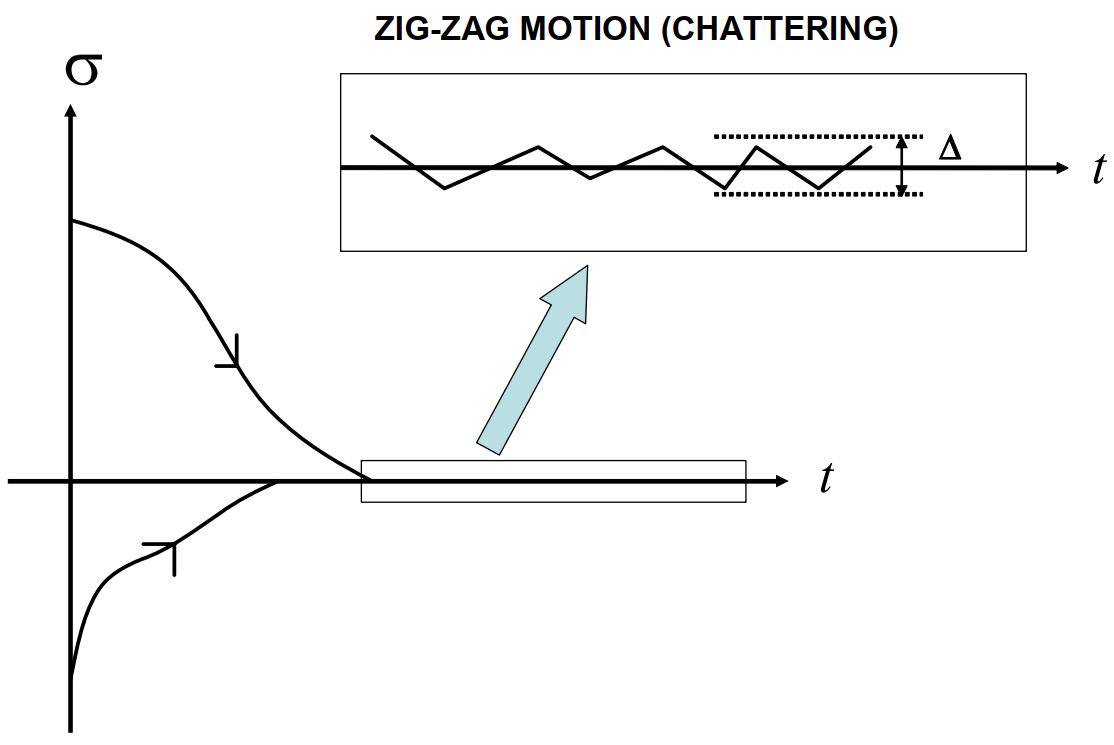
\includegraphics[width=0.6\textwidth]{Images/Control/first_order_sliding_mode_control}
\caption{Typical evolution of $\sigma$ starting from different initial conditions.}
\label{sigma_evolution}
\end{figure}

\begin{figure}[h]
\centering
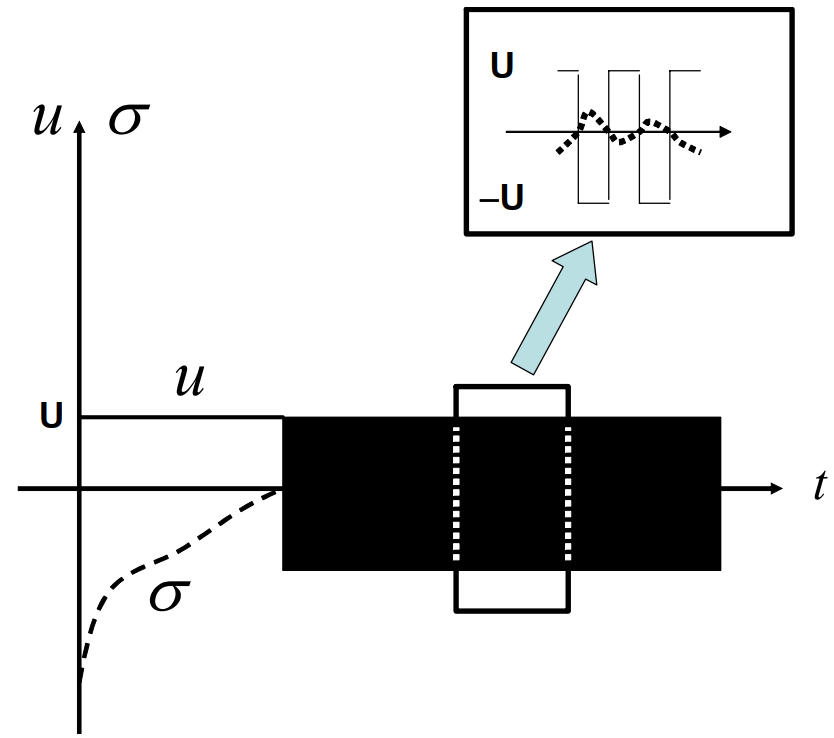
\includegraphics[width=0.6\textwidth]{Images/Control/first_order_sliding_mode_control_b}
\caption{Typical evolution of the control signal $u$ ( $\sigma$ is represented by dashed lines).}
\label{control_evolution}
\end{figure}


\noindent In steady condition the control variable u will alternate at very high (theoretically infinite) frequency along the values u=U
and u=-U, which can be observed in figure \ref{control_evolution}.



\noindent The discontinuous switching control with high frequency  in figure \ref{control_evolution} is suitable in” electrical” implementation (where PWM control signals are usually used) but cause an increase in oscillations and numerous different problems in several areas, such as the control of mechanical systems.


In order to find a solution for the problem presented above (referred to as \textit{”chattering phenomenon”}) roughly (smoothed) execution of sliding mode control techniques have been proposed where the discontinuous \text{“sign”} term is substituted with a  continuous and smooth approximation using one of the two functions below.


\begin{equation}
\begin{aligned}
&\text{SAT} \text{\hspace{1cm}} u=-U sat(\sigma; \epsilon) \equiv -U \frac{\sigma}{|\sigma| + \sigma} \text{\hspace{1.5cm}} \epsilon >0 \text{\hspace{0.5cm}} \epsilon \approx 0 \\
&\text{TANH} \text{\hspace{1cm}} u=-U tanh(\sigma/ \epsilon)  \text{\hspace{3.3cm}} \epsilon >0 \text{\hspace{0.5cm}} \epsilon \approx 0  \\
\end{aligned}
\end{equation}

Unfortunately, this approach is successful only when uncertainties are not applied on the system and the control action that prevents these uncertainties can be set to zero in the sliding mode.


\begin{figure}[h]
\centering
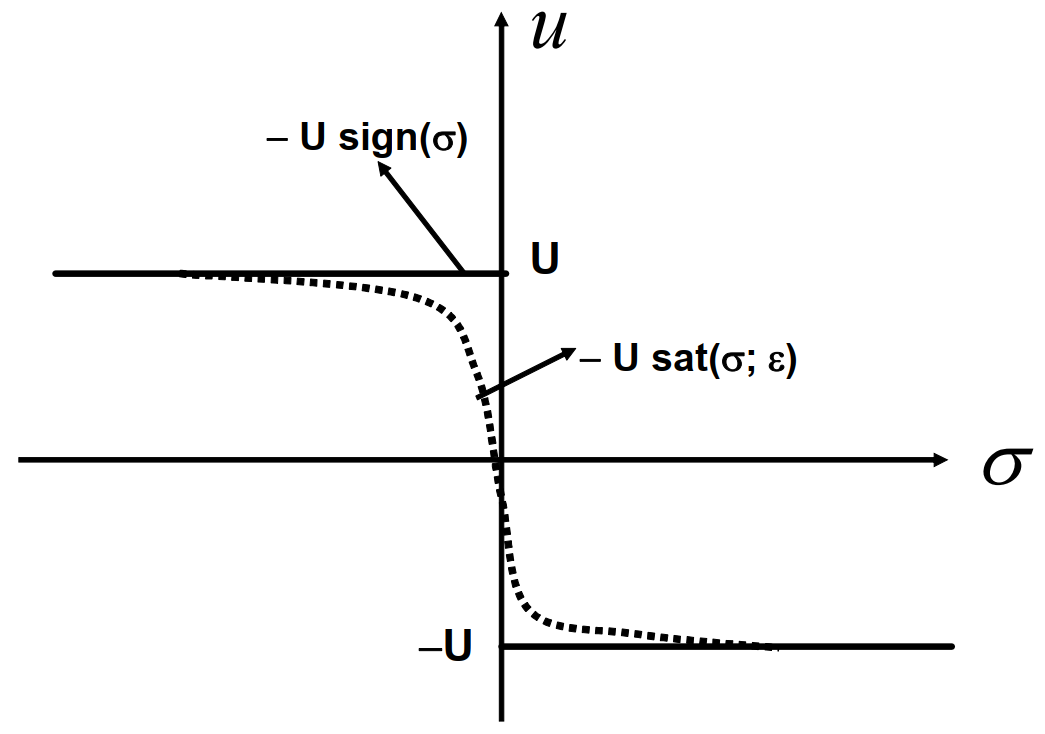
\includegraphics[width=0.6\textwidth]{Images/Control/first_order_sliding_mode_control_c}
\caption{Smooth approximations of sliding mode control.}
\label{Smooth_Sliding_mode_control}
\end{figure}


 
 \subsection{Other types of control}
 
 \chapter{Multi-flips maneuver with quadrotors}
 
 \section{Quadrotor flip physics}
 
 \section{Link to parallel robots}
 
 \section{Control approaches for multi-flip maneuvers}
  
 \chapter{Trajectory optimization} 
 
 \chapter*{Conclusion}
 \addcontentsline{toc}{chapter}{Conclusion}
 
 
 
 


 \addcontentsline{toc}{chapter}{Bibliography}
 \nocite{*}
 
 \bibliography{../biblio}


 
\end{document}
